%% 
%DIF LATEXDIFF DIFFERENCE FILE
%DIF DEL old.tex    Sun Oct 26 10:48:10 2025
%DIF ADD main.tex   Sun Oct 26 10:46:10 2025
%% Copyright 2007-2024 Elsevier Ltd
%% 
%% This file is part of the 'Elsarticle Bundle'.
%% ---------------------------------------------
%% 
\documentclass[preprint,12pt]{elsarticle}

%% Use the option review to obtain double line spacing
%% \documentclass[authoryear,preprint,review,12pt]{elsarticle}

%% Use the options 1p,twocolumn; 3p; 3p,twocolumn; 5p; or 5p,twocolumn
%% for a journal layout:
%% \documentclass[final,1p,times]{elsarticle}
%% \documentclass[final,1p,times,twocolumn]{elsarticle}
%% \documentclass[final,3p,times]{elsarticle}
%% \documentclass[final,3p,times,twocolumn]{elsarticle}
%% \documentclass[final,5p,times]{elsarticle}
%% \documentclass[final,5p,times,twocolumn]{elsarticle}

%% For including figures, graphicx.sty has been loaded in
%% elsarticle.cls. If you prefer to use the old commands
%% please give \usepackage{epsfig}


\usepackage{amssymb}
\usepackage{amsmath}
\usepackage{lineno}
\usepackage[colorinlistoftodos,prependcaption,textsize=tiny]{todonotes}
\journal{Journal of Computer Languages}
%DIF PREAMBLE EXTENSION ADDED BY LATEXDIFF
%DIF UNDERLINE PREAMBLE %DIF PREAMBLE
\RequirePackage[normalem]{ulem} %DIF PREAMBLE
\RequirePackage{color}\definecolor{RED}{rgb}{1,0,0}\definecolor{BLUE}{rgb}{0,0,1} %DIF PREAMBLE
\providecommand{\DIFadd}[1]{{\protect\color{blue}\uwave{#1}}} %DIF PREAMBLE
\providecommand{\DIFdel}[1]{{\protect\color{red}\sout{#1}}} %DIF PREAMBLE
%DIF SAFE PREAMBLE %DIF PREAMBLE
\providecommand{\DIFaddbegin}{} %DIF PREAMBLE
\providecommand{\DIFaddend}{} %DIF PREAMBLE
\providecommand{\DIFdelbegin}{} %DIF PREAMBLE
\providecommand{\DIFdelend}{} %DIF PREAMBLE
\providecommand{\DIFmodbegin}{} %DIF PREAMBLE
\providecommand{\DIFmodend}{} %DIF PREAMBLE
%DIF FLOATSAFE PREAMBLE %DIF PREAMBLE
\providecommand{\DIFaddFL}[1]{\DIFadd{#1}} %DIF PREAMBLE
\providecommand{\DIFdelFL}[1]{\DIFdel{#1}} %DIF PREAMBLE
\providecommand{\DIFaddbeginFL}{} %DIF PREAMBLE
\providecommand{\DIFaddendFL}{} %DIF PREAMBLE
\providecommand{\DIFdelbeginFL}{} %DIF PREAMBLE
\providecommand{\DIFdelendFL}{} %DIF PREAMBLE
%DIF AMSMATHULEM PREAMBLE %DIF PREAMBLE
\makeatletter %DIF PREAMBLE
\let\sout@orig\sout %DIF PREAMBLE
\renewcommand{\sout}[1]{\ifmmode\text{\sout@orig{\ensuremath{#1}}}\else\sout@orig{#1}\fi} %DIF PREAMBLE
\makeatother %DIF PREAMBLE
%DIF COLORLISTINGS PREAMBLE %DIF PREAMBLE
\RequirePackage{listings} %DIF PREAMBLE
\RequirePackage{color} %DIF PREAMBLE
\lstdefinelanguage{DIFcode}{ %DIF PREAMBLE
%DIF DIFCODE_UNDERLINE %DIF PREAMBLE
  moredelim=[il][\color{red}\sout]{\%DIF\ <\ }, %DIF PREAMBLE
  moredelim=[il][\color{blue}\uwave]{\%DIF\ >\ } %DIF PREAMBLE
} %DIF PREAMBLE
\lstdefinestyle{DIFverbatimstyle}{ %DIF PREAMBLE
	language=DIFcode, %DIF PREAMBLE
	basicstyle=\ttfamily, %DIF PREAMBLE
	columns=fullflexible, %DIF PREAMBLE
	keepspaces=true %DIF PREAMBLE
} %DIF PREAMBLE
\lstnewenvironment{DIFverbatim}{\lstset{style=DIFverbatimstyle}}{} %DIF PREAMBLE
\lstnewenvironment{DIFverbatim*}{\lstset{style=DIFverbatimstyle,showspaces=true}}{} %DIF PREAMBLE
\lstset{extendedchars=\true,inputencoding=utf8}

%DIF END PREAMBLE EXTENSION ADDED BY LATEXDIFF

\begin{document}

\begin{frontmatter}

 \author{Shuai Fu}

 \author{Tim Dwyer}

 \author{Peter J. Stuckey}

 \author{John Grundy}


 \affiliation{organization={Monash University}, country={Australia}}


\title{GeckoGraph: A Visual Language for Polymorphic Types}

%% Abstract
\begin{abstract}
Polymorphic \DIFdelbegin \DIFdel{types are }\DIFdelend \DIFaddbegin \DIFadd{type is }\DIFaddend an important feature in most strongly typed programming languages. They allow functions to be written in a way that can be used with different data types, while still enforcing the relationship and constraints between the values. However, programmers often find polymorphic types difficult to use and understand\DIFaddbegin \DIFadd{, }\DIFaddend and tend to reason \DIFdelbegin \DIFdel{using }\DIFdelend \DIFaddbegin \DIFadd{in terms of }\DIFaddend concrete types. We propose GeckoGraph, a graphical notation for types. GeckoGraph aims to \DIFdelbegin \DIFdel{accompany }\DIFdelend \DIFaddbegin \DIFadd{complement }\DIFaddend traditional text-based type notation \DIFdelbegin \DIFdel{and to make }\DIFdelend \DIFaddbegin \DIFadd{by making }\DIFaddend reading, understanding, and comparing types easier. We conducted a large-scale \DIFdelbegin \DIFdel{human study using GeckoGraph compared }\DIFdelend \DIFaddbegin \DIFadd{user study comparing GeckoGraph }\DIFaddend to text-based type notation. To our knowledge, this is the largest controlled user study on functional programming ever conducted. 
The results \DIFdelbegin \DIFdel{of the study show that GeckoGraph helps improve programmers' ability to succeed in the programming tasks we designed, especially for novice programmers. }\DIFdelend \DIFaddbegin \DIFadd{show no overall significant differences in task completion time or success rate. However, we observed a modest improvement in success rate among beginner participants. For the most challenging task, GeckoGraph improved success rates by 14.5\% for beginners and 11.2\% for less experienced users. These findings suggest that GeckoGraph has potential as a teaching and learning aid for polymorphic type systems.
}\DIFaddend \end{abstract}

%% Keywords
\begin{keyword}
%% keywords here, in the form: keyword \sep keyword

%% PACS codes here, in the form: \PACS code \sep code

%% MSC codes here, in the form: \MSC code \sep code
%% or \MSC[2008] code \sep code (2000 is the default)
Polymorphic Types \sep Functional Programming \sep Visual Languages \sep Visualization
\end{keyword}

\end{frontmatter}

\linenumbers

\section{Introduction} \label{sec:intro}
In programming languages, a polymorphic type \cite{Cardelli1987-fp} can represent values of different types while providing an interface to describe common behaviors for those values. Polymorphic types are one of the oldest topics in programming language theory \cite{Cardelli1987-fp}. They are central to the succinctness of \DIFdelbegin \DIFdel{statically-typed languages , }\DIFdelend \DIFaddbegin \DIFadd{statically typed languages }\DIFaddend while also enabling a high degree of type-safe abstraction and reusability. Polymorphic types are available in many programming languages, from functional languages such as Haskell and ML to imperative and multi-paradigm languages such as Rust\cite{Klabnik_undated-wx} and Go\cite{Griesemer_undated-ff}.

% Polymorphism allows programs to be written in a way that is more generic and adaptable to different data types, enabling greater flexibility and code reuse. Polymorphic types are ideal for modeling abstractions, such as properties of mathematical objects and laws that hold on these objects. 

While promoting robustness and code reusability, polymorphic types present challenges in learning and comprehension, particularly for novice users \cite{Jun2000-ec, Jun2000-yu}; as it is often argued that the expressiveness \DIFdelbegin \DIFdel{power }\DIFdelend of type systems often comes at the cost of their usability~\cite{Hage2020-hg}. Research indicates that humans tend to focus on concrete types and rely on polymorphic type checking only as a last resort. Moreover, polymorphic types often complicate \DIFdelbegin \DIFdel{type error usability }\DIFdelend \DIFaddbegin \DIFadd{the usability of type errors}\DIFaddend . During type checking, compilers frequently generate new polymorphic type variables temporarily. These variables are typically discarded after type checking unless a type error occurs, in which case they are referenced in error messages. Consequently, programmers often face the task of resolving type errors involving type variables they did not explicitly author (Fig. \ref{fig:example-foldable}). Unfortunately, not many \DIFdelbegin \DIFdel{research focuses }\DIFdelend \DIFaddbegin \DIFadd{studies focus }\DIFaddend on the \textit{usability} of polymorphic types. 

\begin{figure}[]
  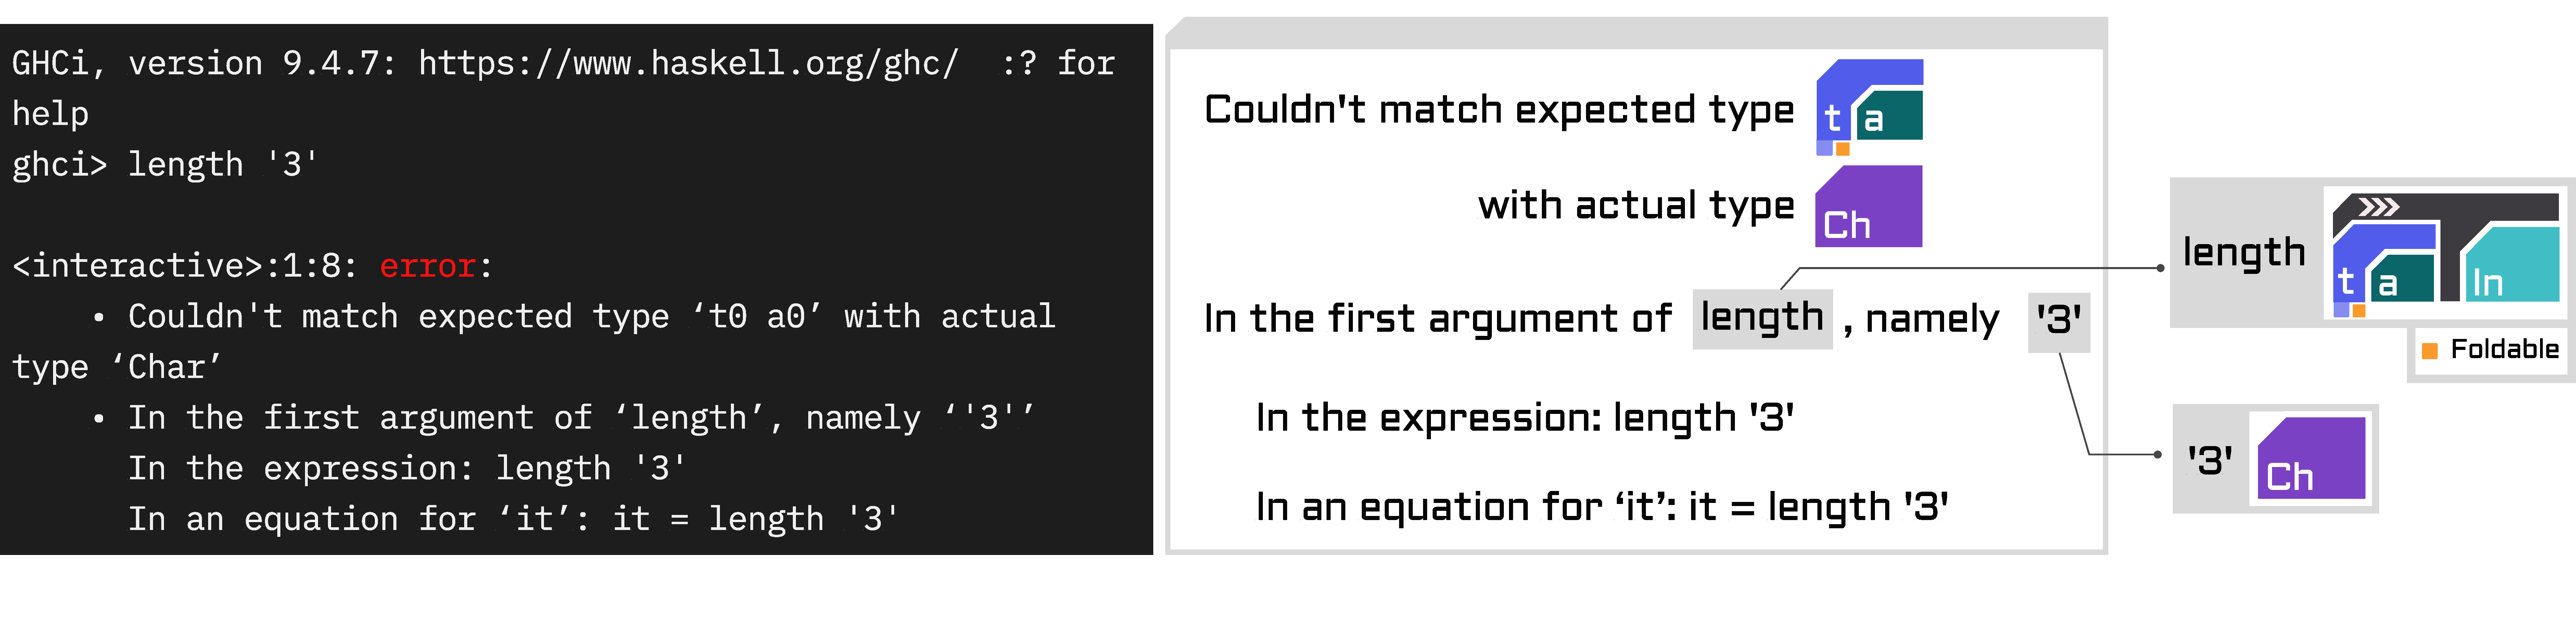
\includegraphics[width=\linewidth]{figures/Foldable}
  \caption{\label{fig:example-foldable} An example type error where a programmer mistakenly provided a \texttt{Char} instead of a \texttt{String} literal. \DIFdelbeginFL \textbf{\DIFdelFL{Left --}} %DIFAUXCMD
\DIFdelFL{The compiler shows an error message comparing the provided Char }\DIFdelendFL \DIFaddbeginFL {\bf \DIFaddFL{Left:}} \DIFaddFL{Original }\DIFaddendFL type \DIFdelbeginFL \DIFdelFL{to a confusingly named type }\texttt{\DIFdelFL{t0 a0}}%DIFAUXCMD
\DIFdelendFL \DIFaddbeginFL \DIFaddFL{error}\DIFaddendFL . \DIFdelbeginFL \textbf{\DIFdelFL{Right --}} %DIFAUXCMD
\DIFdelFL{GeckoGraph shows the exact message }\DIFdelendFL \DIFaddbeginFL {\bf \DIFaddFL{Right:}} \DIFaddFL{Type error }\DIFaddendFL with \DIFdelbeginFL \DIFdelFL{the two types in graphic notation, highlighting the structural difference rather than identifier names.}\DIFdelendFL \DIFaddbeginFL \DIFaddFL{GeckoGraph}\DIFaddendFL }
\end{figure}

 We aim to investigate the challenges of using polymorphic types and explore how to improve their usability with visualization and modern Human-Computer Interaction (HCI) techniques. In this paper, we propose GeckoGraph, a graphical notation for types. GeckoGraph aims to complement traditional text-based type notation and make reading, understanding, and comparing types easier. GeckoGraph is prototyped and \DIFdelbegin \DIFdel{verified iteratively , leading to }\DIFdelend \DIFaddbegin \DIFadd{iteratively verified, resulting in }\DIFaddend a design with visual clarity applicable \DIFdelbegin \DIFdel{to }\DIFdelend \DIFaddbegin \DIFadd{across }\DIFaddend many programming contexts. 
 \DIFdelbegin \DIFdel{We designed an online puzzle game }\textit{\DIFdel{ZeroToHero}}%DIFAUXCMD
\footnote{\DIFdel{Available at https://zerotohero.fly.dev}}%DIFAUXCMD
\addtocounter{footnote}{-1}%DIFAUXCMD
\DIFdel{, evaluating 714 participants' performance to solve a series of programming challenges using GeckoGraph versus }\DIFdelend \DIFaddbegin \DIFadd{To evaluate its effectiveness, we conducted a large-scale user study comparing GeckoGraph with standard }\DIFaddend text-based type \DIFdelbegin \DIFdel{annotation, which is, to }\DIFdelend \DIFaddbegin \DIFadd{notation. To }\DIFaddend our knowledge, \DIFaddbegin \DIFadd{this represents }\DIFaddend the largest controlled user study \DIFdelbegin \DIFdel{of a functional programming tool or concept.
The study results show that GeckoGraph helps improve programmers ' ability to succeed in resolving programming challenges, especially for novice programmers}\DIFdelend \DIFaddbegin \DIFadd{on functional programming to date.
The results show no overall significant differences in task completion time or success rate. However, we observed a modest improvement in success rate among beginner participants. For the most challenging task, GeckoGraph improved success rates by 14.5\% for beginners and 11.2\% for less experienced users. These findings suggest that GeckoGraph has potential as a teaching and learning aid for polymorphic type systems.
}

%DIF >  In Section~\ref{sec:type-systems}, we review key type system features in functional programming languages, many of which have recently been adopted by object-oriented and multi-paradigm languages. We highlight how these features enable flexible abstraction and expressive type modeling, while sometimes hindering usability for beginners. Section~\ref{sec:gecko-graph} presents the design of GeckoGraph, illustrating how it visualizes complex type-level information that is often implicit or hard to interpret textually. Section~\ref{sec:evaluation} describes our user study, ZeroToHero, a series of 10 programming challenges, along with the study design, recruitment, and hypotheses. Section~\ref{sec:results} reports quantitative and qualitative findings, including completion time, success rates, and participant feedback. In Section~\ref{sec:discussion}, we interpret these results, discuss GeckoGraph’s benefits and usability challenges, and explore potential applications. Section~\ref{sec:related-work} reviews related visualization research, and Section~\ref{sec:conclusion} summarizes our contributions and outlines future directions.

\section{\DIFadd{Type Systems in Functional Programming}} \label{sec:type-systems}

\DIFadd{Functional programming languages have a rich history of embracing strong type systems and pioneering advanced type system features \mbox{%DIFAUXCMD
\cite{Milner1978-ob, MacQueen2020-qn, Hudak2007-kn}}\hskip0pt%DIFAUXCMD
. In functional programming languages, type systems are often more expressive and provide stronger safety guarantees. They enable programmers to model program behavior rigorously and enforce correctness at compile time. Common characteristics of type systems in functional programming include structural typing, algebraic data types, parametric polymorphism, and type inference.
}

{\bf \DIFadd{Structural typing}} \DIFadd{is often the primary approach for determining type equivalence and compatibility in functional programming languages (e.g., Elm and OCaml) and multi-paradigm languages (e.g., TypeScript). In contrast, nominal type systems are often predominant in Object-Oriented languages such as Java and C\# \mbox{%DIFAUXCMD
\cite{AbdelGawad2013-hh}}\hskip0pt%DIFAUXCMD
. In nominal systems, two types are considered distinct even if they have identical structure but different names. In contrast, structural type systems consider types equivalent as long as their structures match, regardless of their names. This approach promotes flexibility, as types can be defined inline without introducing new names, and values are automatically valid for a type when they conform to the structure.  However, this lack of nominality can also make complex types harder to read and reason about. For instance, when encountering type errors, programmers can face two mismatched types with a complex structure, and understanding where exactly the root error is becomes a tedious task of string comparison (Fig. \ref{fig:structural}).
}

\begin{figure}[]
  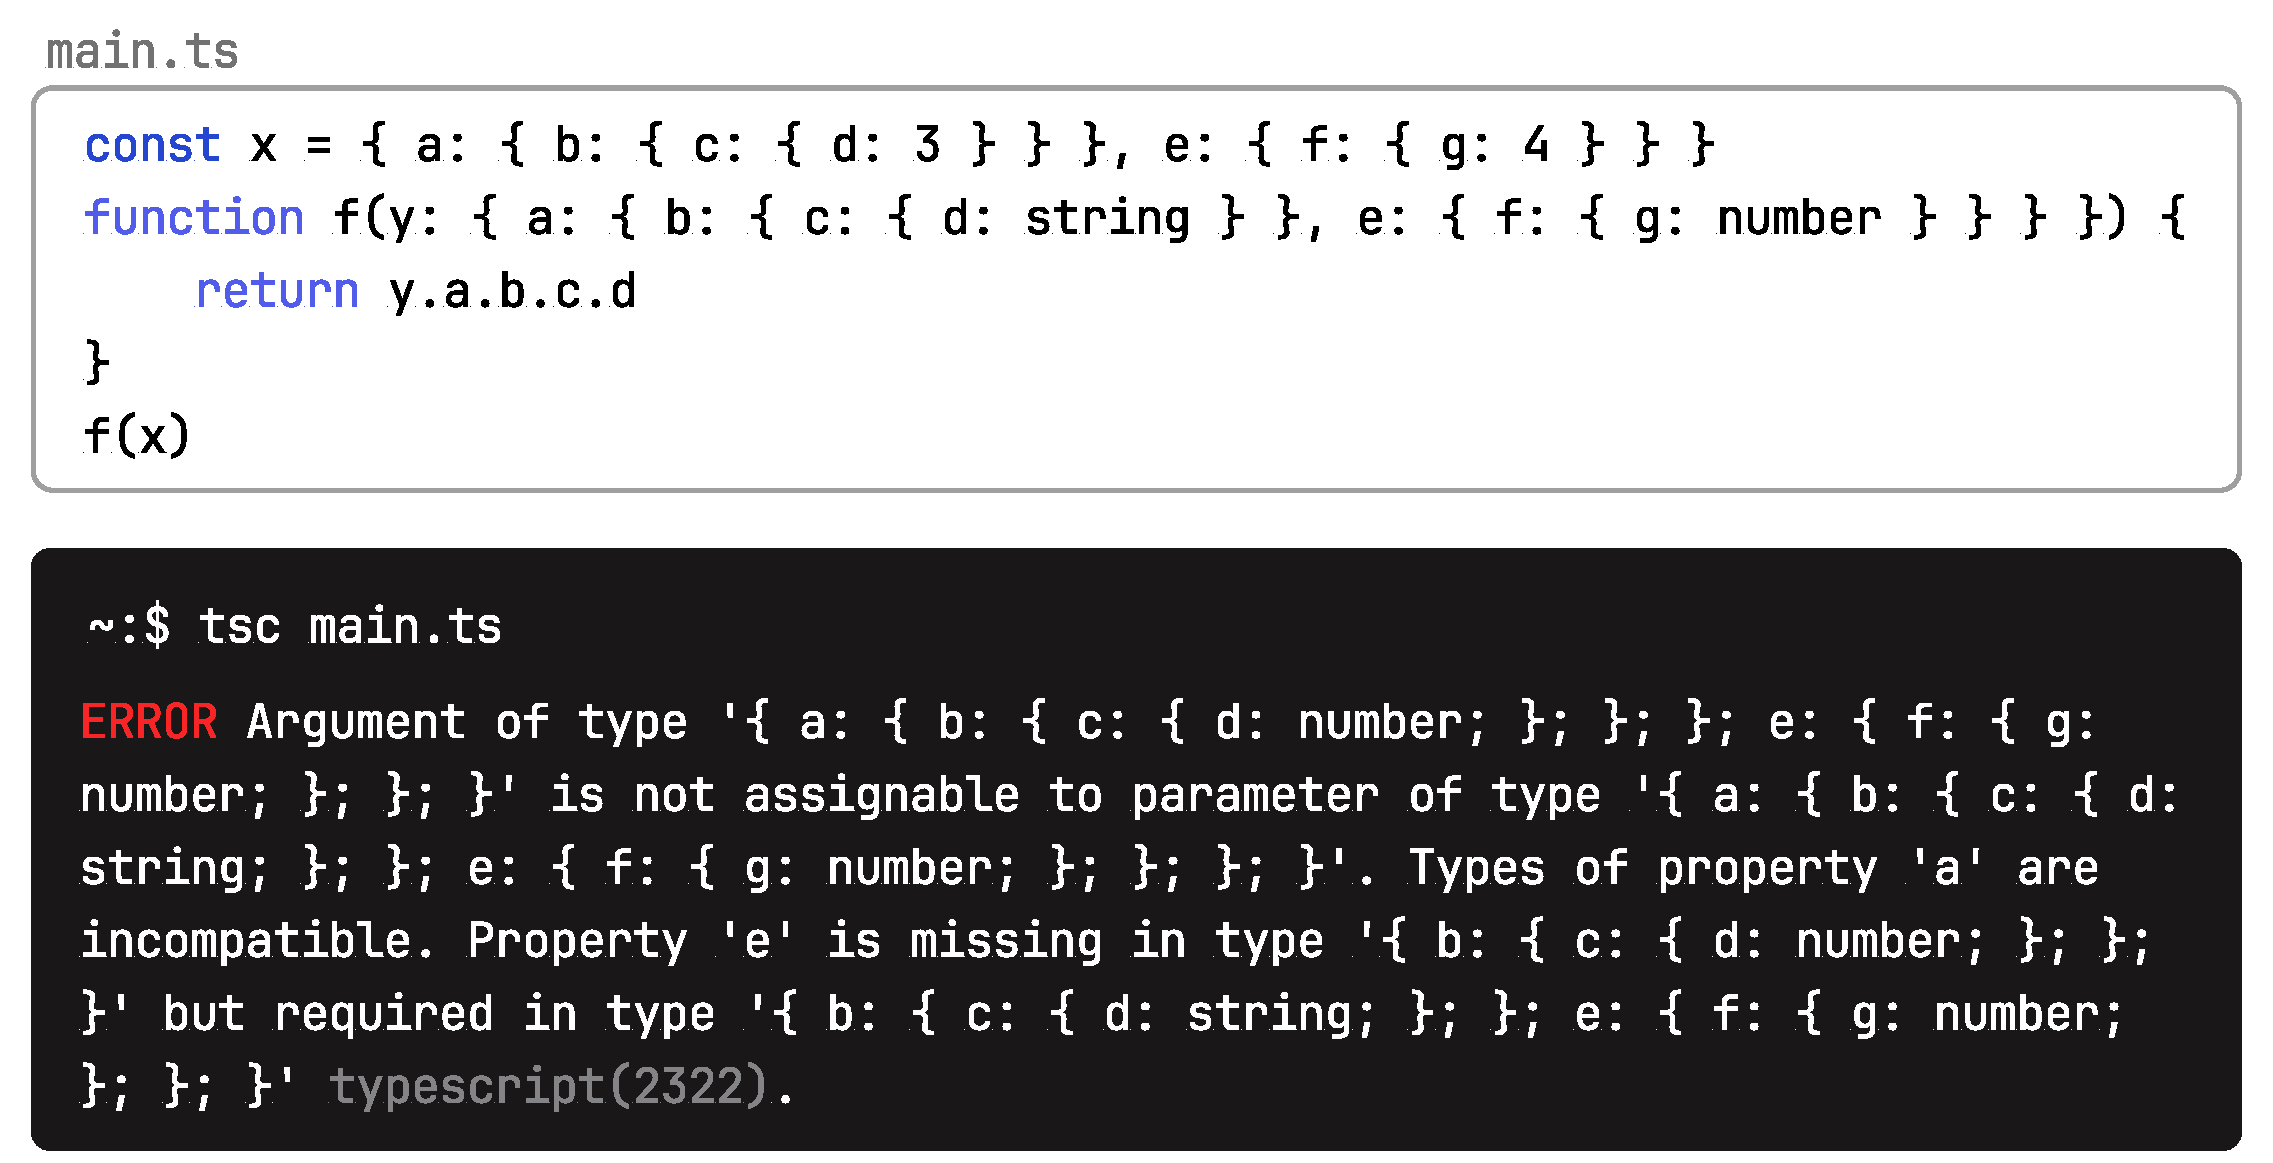
\includegraphics[width=\linewidth]{figures/structural}
  \caption{\label{fig:structural} \DIFaddFL{Example of a TypeScript structural type error. (Top) The function }\texttt{\DIFaddFL{f}} \DIFaddFL{expects a parameter with a string field }\texttt{\DIFaddFL{d}}\DIFaddFL{, but the argument }{\tt \DIFaddFL{x}} \DIFaddFL{provides a numeric }{\tt \DIFaddFL{d}}\DIFaddFL{. (Bottom) The error message is dreadful to read.}}
\end{figure}

{\bf \DIFadd{Algebraic data types}} \DIFadd{(ADTs) \mbox{%DIFAUXCMD
\cite{Milner1978-qz} }\hskip0pt%DIFAUXCMD
allow developers to construct complex types from simpler ones using sum and product operations. A }{\bf \DIFadd{sum type}}\DIFadd{, often called a tagged union, $A + B$, represents a type that can be a value of A or a value of B. Conversely, a }{\bf \DIFadd{product type}} \DIFadd{$A \times B$ represents a tuple type composed of two values of both }{\tt \DIFadd{A}} \DIFadd{and }{\tt \DIFadd{B}}\DIFadd{. This formalization allows precise and composable type construction for common data structures such as lists, tuples, and result types.
For example, in Haskell, types like }\texttt{\DIFadd{data Either a b = Left a | Right b}} \DIFadd{and }\texttt{\DIFadd{data Maybe a = Nothing | Just a}} \DIFadd{provide basic building blocks for error handling, and the type }\texttt{\DIFadd{data List a = }[] \DIFadd{| a : List a }} \DIFadd{provides a succinct recursive definition for lists. This illustrates the expressive power of ADTs. However, in practice, type definitions can grow to be complex structures, for instance }\texttt {\DIFadd{Maybe (Either }[\DIFadd{Maybe a}] \DIFadd{(Either a String))}} \DIFadd{as programs grow, causing difficulties to interpret and maintain. 
}


{\bf \DIFadd{Parametric polymorphism}} \DIFadd{(often called generics) allows functions and data structures to operate uniformly across different types. For instance, in Haskell, the function }\texttt{\DIFadd{head :: }[\DIFadd{a}] \DIFadd{-> a}}\DIFadd{, taking a list as input and returning the first element, is a polymorphic function that works on lists of any type; integers, strings, and functions are all valid candidates for the generic variable }\texttt{\DIFadd{a}}\DIFadd{.  It provides a strong and principled form of abstraction, enabling code reuse without sacrificing type safety.
}

\DIFadd{However, parametric polymorphism also increases cognitive load: programmers must mentally track type variables and reason about how concrete types are instantiated during function application. This task becomes more challenging when functions involve multiple type variables. An example would be the foldM function: }\texttt{\DIFadd{foldM :: (Monad m) => (a -> b -> m a) -> a -> }[\DIFadd{b}] \DIFadd{-> m a}}\DIFadd{. The challenge of reading and understanding polymorphic types is more serious for novice users \mbox{%DIFAUXCMD
\cite{Jun2000-ec, Jun2000-yu}}\hskip0pt%DIFAUXCMD
.
}



{\bf \DIFadd{Type inference}}\DIFadd{, or implicit typing, reduces the need for explicit type annotations by allowing the compiler to deduce types automatically.
Most modern languages employ some level of inference. For instance, Java’s var keyword (introduced in version 10) infers variable types at compile time based on their assigned values \mbox{%DIFAUXCMD
\cite{Java_Developers2023-an}}\hskip0pt%DIFAUXCMD
, saving programmers from writing redundant type declarations, such as }\textit {\DIFadd{Car car = new Car()}}\DIFaddend .

\DIFaddbegin \DIFadd{Functional languages such as Haskell and ML go further, using global type inference \mbox{%DIFAUXCMD
\cite{Damas1982-zw} }\hskip0pt%DIFAUXCMD
to check entire programs without requiring explicit annotations. While this improves conciseness, it can reduce code readability and produce complex error messages. Many programmers, therefore, choose to write explicit type signatures for clarity, even when inference is available.
}




{\it \DIFadd{To summarize}}\DIFadd{, the type systems of functional programming languages provide rigorous tools for specifying and enforcing program behavior. By encoding system constraints directly in types, they prevent many classes of runtime errors. However, this rigor introduces trade-offs: a steeper learning curve and less flexibility for exploratory or prototype development. In the following sections, we explore how GeckoGraph supports these type-system features by visualizing type-level information that is often implicit or difficult for humans to interpret.
}


\DIFaddend \section{GeckoGraph} \DIFaddbegin \label{sec:gecko-graph}
\DIFaddend 

GeckoGraph is a visual notation for type annotations in statically typed programming languages. It is intended to work tangibly with text-based annotations but uses colors, shapes, and symbols to make structures of types easy to identify at a glance. In this section, we describe the design of GeckoGraph and highlight some unique benefits of programming with GeckoGraph.

\subsection{Design of GeckoGraph}
The design of GeckoGraph focuses on visualizing types in functional languages (e.g., Haskell, ML). In this paper, we use Haskell as an example. As illustrated in this section, it can express basic types, polymorphic types, algebraic data types, \DIFdelbegin \DIFdel{and many }\DIFdelend \DIFaddbegin \DIFadd{type classes, and a few }\DIFaddend advanced type-level features. However, GeckoGraph \DIFdelbegin \DIFdel{could }\DIFdelend \DIFaddbegin \DIFadd{can }\DIFaddend also be used in imperative and multiparadigm languages such as TypeScript and Rust. We provide a GeckoGraph visualization tool available online for multiple languages \cite{Fu2025-ka}.

We identified three main design goals for GeckoGraph based on the challenges of using polymorphic types~\cite{Jun2000-ec, Jun2000-yu} and how programmers tend to use type annotations to support their programming tasks~\cite{Justin_Lubin2021-yy}, as follows. 

\paragraph{\textbf{(D1) Easy to learn}}\label{goal1} GeckoGraph should take little to no effort to learn. The rules to translate a text-based type notation to GeckoGraph should be minimal. Where possible, GeckoGraph should be intuitive to programmers who are familiar with text-based type notation.

\begin{figure}[!h]
  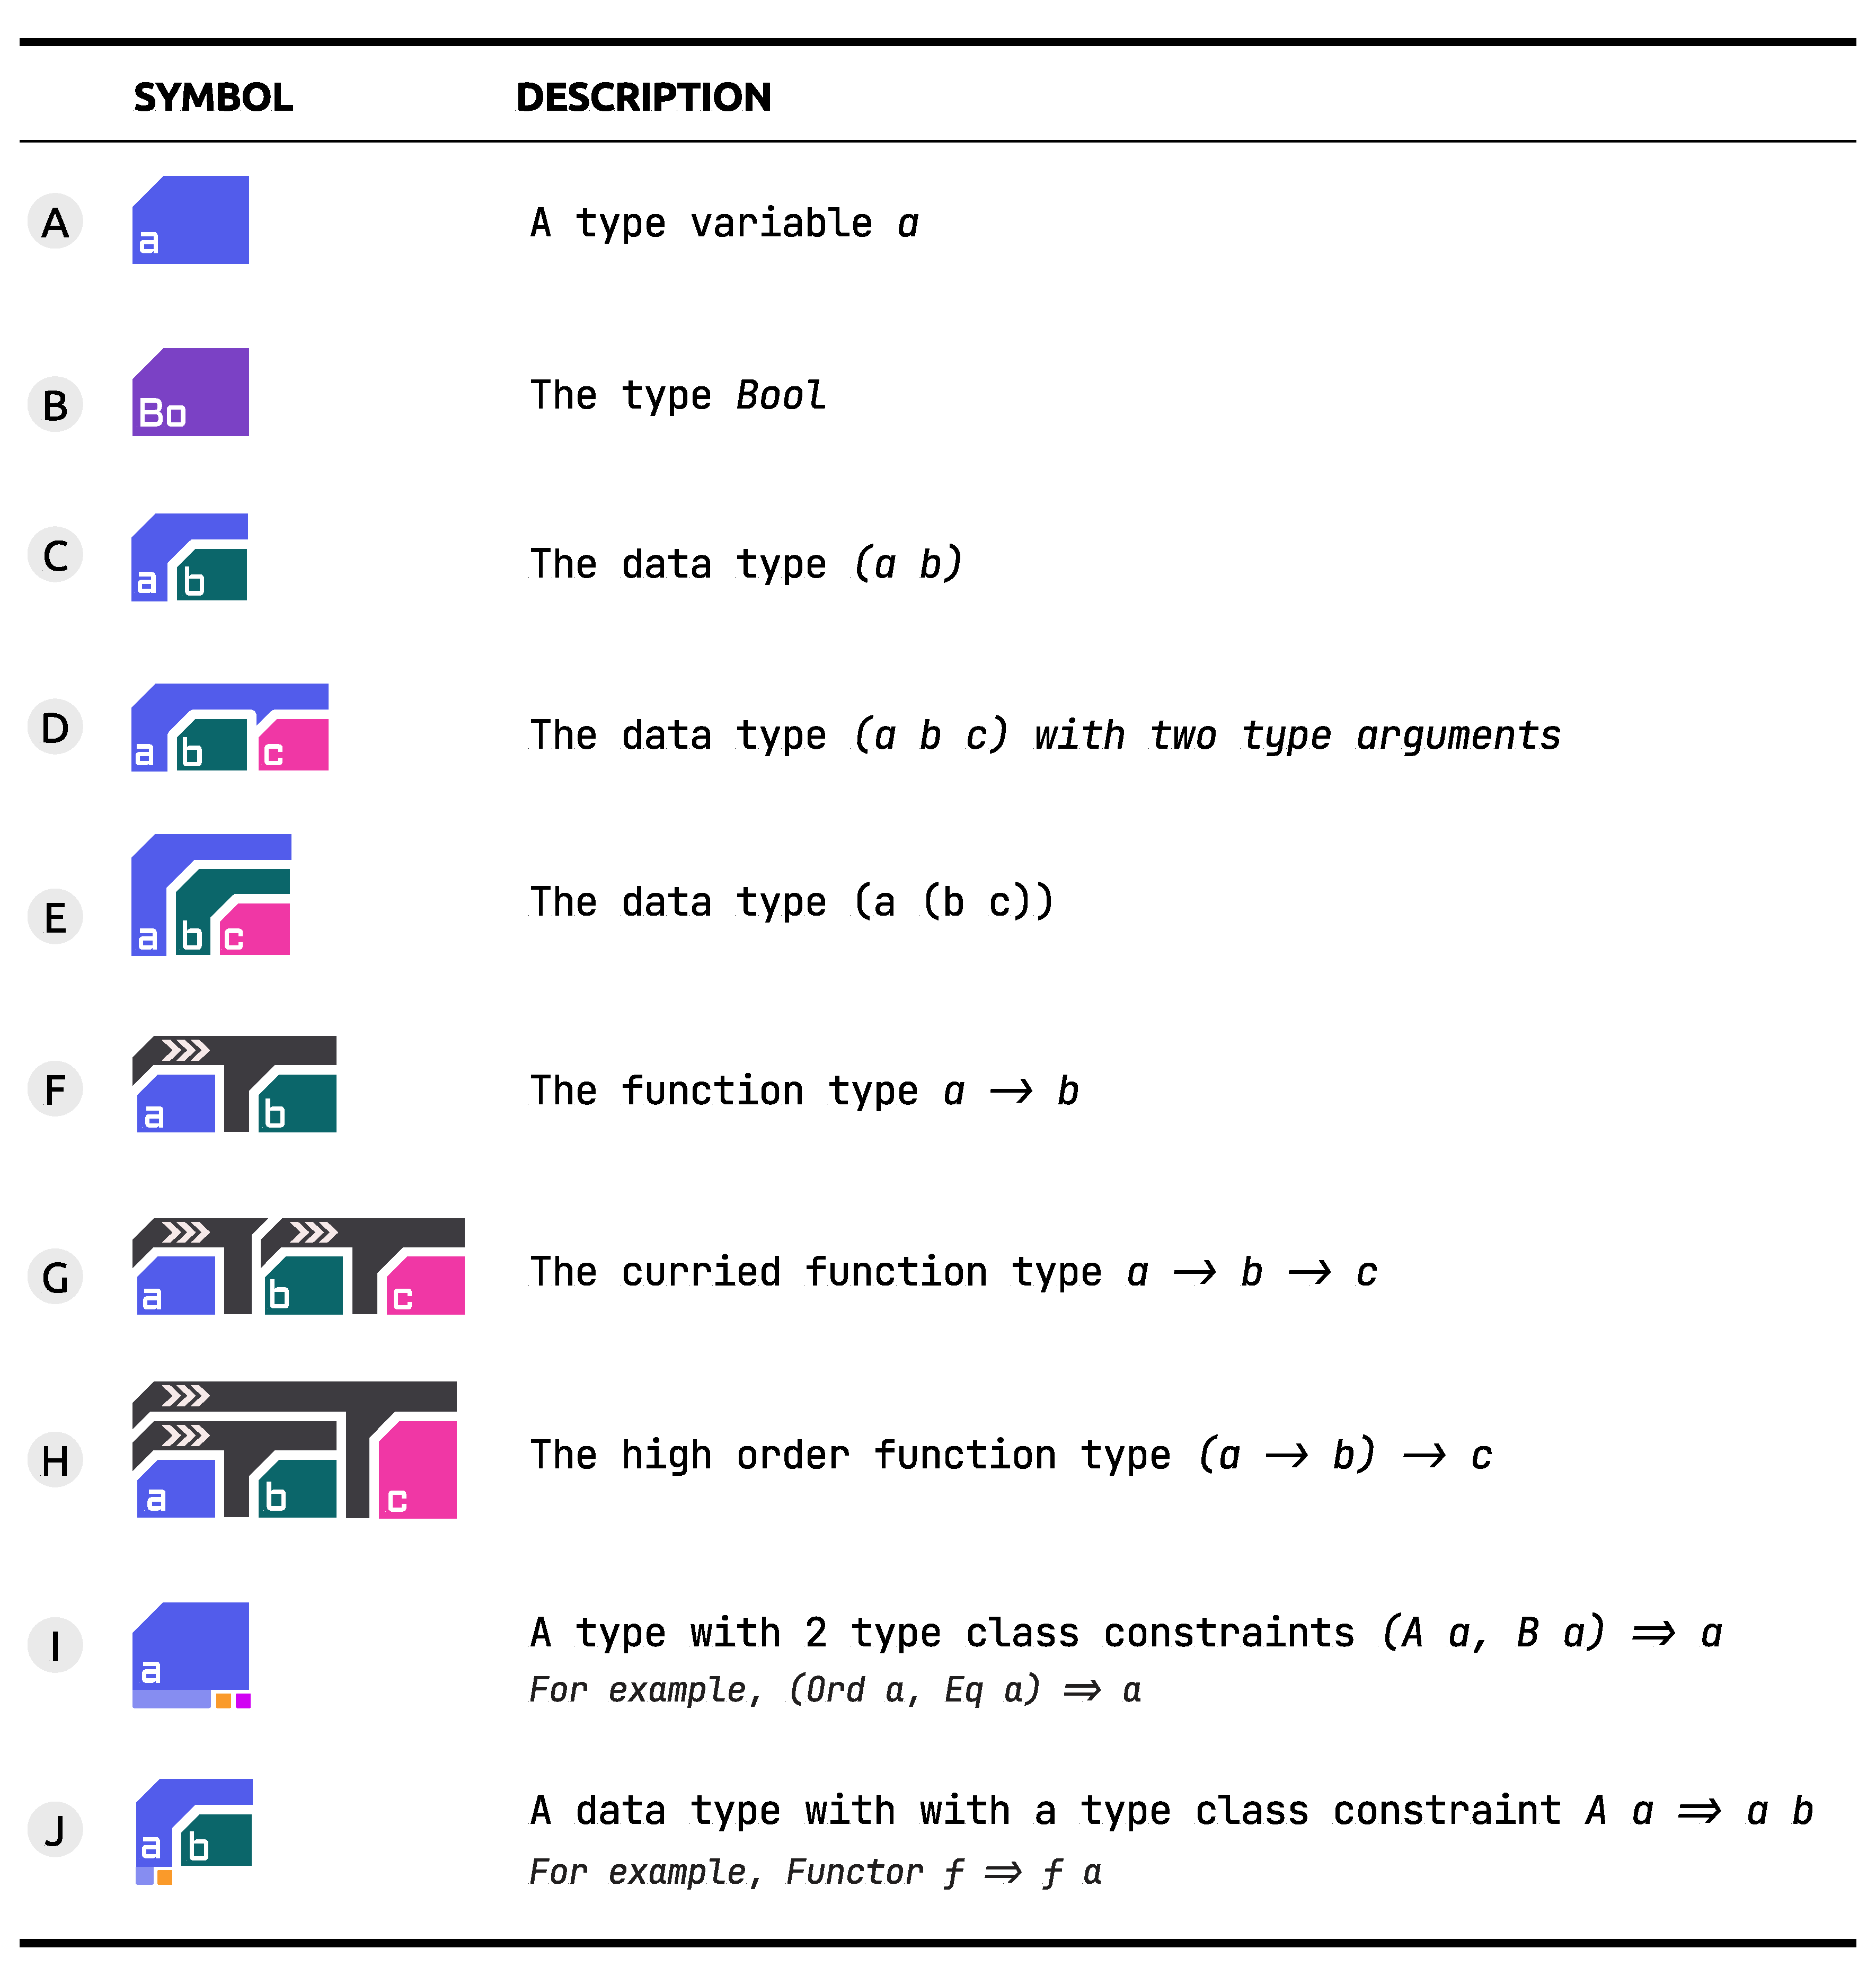
\includegraphics[width=\linewidth]{figures/Design}
  \caption{
        \label{fig:design}
        Examples of various types as represented in GeckoGraph, including type variables (A) and concrete types (B). Data types (C, D, E), function types (F, G, H), and type classes (I, J).
  }
\end{figure}

\paragraph{\textbf{(D2) Easy to parse for humans}}  \label{goal2} GeckoGraph should make the task of reading and understanding type notation easy. It should emphasize the less obvious properties of a type signature. GeckoGraph should eliminate the need for mental backtracking, such as counting opening and closing parentheses and remembering which type classes are required on which variables. 

\paragraph{\textbf{(D3) Optimized for comparing and searching}} \label{goal3} GeckoGraph aims to make the task of comparing two types easy, especially to make subtle differences in text-based notation harder to miss. This also includes the task of choosing an ideal function from a list of potential functions. For example, programmers search for a desired function from a documentation site with only partial knowledge of its type (e.g., the arity of a function, containing a known type, or type class requirements). 

\DIFaddbegin \DIFadd{Motivated by the design goals, we designed GeckoGraph with the following features and construction rules (Fig. \ref{fig:design}):
}

\DIFaddend \paragraph{Simple Types} 
Simple types, such as type variables and concrete types, are displayed in a cell \includegraphics[height=1em]{figures/SimpleType}: a solid-colored rectangular box with an angled corner on the top left. Each type identifier encodes a distinct color hue of the cell. Its first 1 or 2 letters are displayed inside the cell at the bottom left to provide familiarity (design goal \ref{goal1}) and a strong secondary encoding. The angled corner in the top left provides visual separation between two cells, even when the same color cells are next to each other, allowing GeckoGraph to be zoomed out to extremely small sizes (Section \ref{subsec:space}) without suffering readability (design goal \ref{goal2}).



\paragraph{\DIFdelbegin \DIFdel{Complex types}\DIFdelend \DIFaddbegin \DIFadd{Algebraic Data Types}\DIFaddend }
GeckoGraph displays an algebraic data type as a larger cell, where the type constructor half encloses its arguments: \includegraphics[height=1em]{figures/DataType.png}. The arguments are aligned in the bottom right of the cell. Two distinct visual dimensions are used to provide additional visual clarity (design goal \ref{goal2}). Data types containing more arguments (e.g., \texttt{ a b c} or \texttt{(a b) c}) will expand horizontally \includegraphics[height=1em]{figures/DataTypeWide.png}. Data types that are nested (e.g. \texttt{ a (b c)}) will grow taller \includegraphics[height=1.2em]{figures/DataTypeNested.png}. This distinction accommodates our design goal \ref{goal3}. Note that the height of GeckoGraph grows only upwards, but not downwards. Not only does this allow GeckoGraph to be more efficient in its space usage, but it also allows the legend text to be consistently aligned at the bottom and can be read as though it is a text-based type notation (design goal \ref{goal1}).  

\paragraph{Function Types}
Functions are the fundamental building blocks of functional programming languages, and function types are ubiquitous and the most important in type-level programming. In Haskell, \texttt{(->)} is defined as an infix type operator with \DIFdelbegin \DIFdel{the }\DIFdelend right associativity to provide succinct type \DIFdelbegin \DIFdel{annotation}\DIFdelend \DIFaddbegin \DIFadd{annotations}\DIFaddend . GeckoGraph preserves this syntax feature to make the notation more intuitive (design goal \ref{goal1}): the 2 arguments of a function type in GeckoGraph are placed on both sides of the cell \includegraphics[height=1em]{figures/Function.png}. A special function indicator (\texttt{$>>>$}) is displayed at the top of the cell. 

Curried functions (e.g., \texttt{ a -> b -> c}) are displayed as two cells of functions merged together \includegraphics[height=1em]{figures/Curry.png}. It appears as if the second function covers the right half of the first function, indicating that the second function is the return type of the first. Regular high-order functions (e.g., \texttt{(a -> b) -> c}) follow the rules of functions and nested data types \includegraphics[height=1.2em]{figures/HOF.png}. The placement of function indicators aims to make it easy to find desired functions in the documentation site based on function arity and \DIFdelbegin \DIFdel{high-order }\DIFdelend \DIFaddbegin \DIFadd{higher-order }\DIFaddend functions (design goal \ref{goal3}). It is easy to tell high-order functions from the vertical position of \DIFdelbegin \DIFdel{its function indicator}\DIFdelend \DIFaddbegin \DIFadd{the function indicators}\DIFaddend . Similarly, it is easy to count the arity of a function by counting the number of \DIFdelbegin \DIFdel{horizontally connected function indicators (}\DIFdelend \DIFaddbegin \DIFadd{function indicators at the outer layer. For example, in }\DIFaddend Fig. \ref{fig:indicator}\DIFdelbegin \DIFdel{). 
}\DIFdelend \DIFaddbegin \DIFadd{, the outer layer function indicators (the ones colored in the lightest shade of gray) suggest a ternary function. The two argument types and the return type are all functions.
}\DIFaddend 

\begin{figure}[h]
  \includegraphics[width=\linewidth]{figures/Indicator}
  \caption{
        \label{fig:indicator}
        An example of \DIFaddbeginFL \DIFaddFL{the }\DIFaddendFL visual hierarchy of the function indicator. The function indicator can be used to easily identify the arity of a function type by counting the connecting function indicators. For higher-order functions where functions are arguments or return values of other functions, it is very easy to see the ``level" of functions. 
  }
\end{figure}

 
\paragraph{Type Classes} 
Type classes are an intrinsic part of Haskell \cite{Hudak2007-kn}, and many other functional languages. In GeckoGraph, the type classes (e.g., \texttt{ (A a, B a) => a}) are indicated in the extended area below one or more GeckoGraph cells \includegraphics[height=1.2em]{figures/TypeClass.png}. Each type class required on a type variable displays as a square indicator aligned on the right of the extended area. In GeckoGraph, a type-class \DIFdelbegin \DIFdel{gliph }\DIFdelend \DIFaddbegin \DIFadd{glyph }\DIFaddend is embedded in every type variable that requires this class. This means when displaying the type \texttt{(==) :: Eq a => 
a -> a -> Bool} in GeckoGraph, the constraint \texttt{Eq} appears in twice on both occurrences of the type variable \texttt{a}. 

The GeckoGraph type class's design promotes the type class placements rather than the type class names. Programmers can easily see where and how many type classes are required, but they may need an extra step (global legends of the color mapping or \DIFaddbegin \DIFadd{a }\DIFaddend pop-up window) to identify the name of the type class. We believe that this is a well-justified trade-off. The strength of this approach lies in situations when \DIFaddbegin \DIFadd{the }\DIFaddend type class context is complex. When reading a type \texttt{(A a, A c, B a, B b, C b) => a -> b -> c}, programmers may need to switch back and forth to remember which type classes are needed on which variable. \DIFdelbegin \DIFdel{GeckoGraph uses approximity to help minimize the }\DIFdelend \DIFaddbegin \DIFadd{In GeckoGraph, type classes are explicitly displayed under the type variable cell,  minimizing programmers' }\DIFaddend effort to associate each type variable with all its type classes (design goal \ref{goal2}). 


\subsection{Key Design Criteria of GeckoGraph}\label{sec:benefits}

GeckoGraph was designed through many different iterations. Many research methods were used to verify ideas, including prototyping, cognitive walk-throughs, and formative studies. We discuss some notable visual dimensions in GeckoGraph and their justifications.


\DIFdelbegin %DIFDELCMD < \begin{figure}[]
%DIFDELCMD <   \includegraphics[width=\linewidth]{figures/PreviousVersions}
%DIFDELCMD <   %%%
%DIFDELCMD < \caption{%
{%DIFAUXCMD
%DIFDELCMD < \label{fig:previous}%%%
\DIFdelFL{Previous Versions of GeckoGraph. Different encodings represent named types, type variables, type constructors, and high-order functions.}}
%DIFAUXCMD
%DIFDELCMD < \end{figure}
%DIFDELCMD < 

%DIFDELCMD < %%%
\DIFdelend \paragraph{Visual Dimensions of GeckoGraph}
\DIFaddbegin 

\DIFaddend \textbf{The colors of GeckoGraph} help programmers to see the permutation of type variables in the input and output of a function. A recent review \cite{Zeng2023-jz} of 59 graphical perception articles showed that combining solid color hue in a filled shape provides stronger visual perception for nominal data such as type identifiers. \DIFdelbegin \DIFdel{Goanna }\DIFdelend \DIFaddbegin \DIFadd{GeckoGraph uses }\DIFaddend a qualitative color scheme from ColorBrewer \cite{Harrower2003-vu} \DIFaddbegin \DIFadd{to encode symbolic values of types}\DIFaddend . One example of GeckoGraph's use of color is the ``rotation" function  (Fig. \ref{fig:rotate}) in the user study (Section \ref{sec:evaluation}). With text-based type notation, programmers often rely on mnemonic devices such as alphabetic ordering or naming conventions. For example, the rotation function \texttt{f2 :: Zero a b c d -> Zero b c d a} \DIFdelbegin \DIFdel{in the game. It }\DIFdelend \DIFaddbegin \DIFadd{appeared in the evaluation (Section \ref{sec:evaluation}), }\DIFaddend shuffles the type arguments one step to the left. The purpose of this function becomes less recognizable if changed to \texttt{f2 :: Zero e v m h -> Zero v m h e}. 

\begin{figure}[]
  \includegraphics[width=0.6\linewidth]{figures/rotate}
  \caption{\label{fig:rotate} The `\DIFdelbeginFL \DIFdelFL{rotate}\DIFdelendFL \DIFaddbeginFL \DIFaddFL{f2}\DIFaddendFL ' function in the user study. \DIFdelbeginFL \DIFdelFL{The name given in the game is `f2'. }\DIFdelendFL It shuffles the type arguments one step to the left\DIFaddbeginFL \DIFaddFL{, and the leftmost argument wraps around to be the rightmost}\DIFaddendFL .}
\end{figure}

\textbf{The horizontal axis of GeckoGraph} \DIFdelbegin \DIFdel{often are helpful in }\DIFdelend \DIFaddbegin \DIFadd{is often helpful for }\DIFaddend identifying differences in function arities. For example, in Fig. \ref{fig:add3}, the programmer intended to implement a function that sums 3 integers. In the implementation, the programmer missed a \texttt{(+)} function at the end; the resulting function type is largely different in length. It is also clear that the function needs to apply to one more binary function to satisfy the length requirement.  

\DIFdelbegin %DIFDELCMD < \begin{figure}[]
%DIFDELCMD <   %%%
\DIFdelendFL \DIFaddbeginFL \begin{figure}[h]
  \DIFaddendFL \includegraphics[width=0.6\linewidth]{figures/Add3}
  \caption{\label{fig:add3} An implementation of function \texttt{add3} but the author missed an (+) from the correct implementation (.) ((+) .) (+). GeckGraph highlights the difference in arity and reveals that a binary function is needed on the right-hand side for the arity to match. }
\end{figure}

\textbf{The vertical axis of GeckoGraph} often helps identify the number of levels in a nested complex type. This can often be very useful when inspecting \DIFdelbegin \DIFdel{mismatching type errors }\DIFdelend \DIFaddbegin \DIFadd{mismatched types }\DIFaddend where data types are nested \DIFdelbegin \DIFdel{in }\DIFdelend \DIFaddbegin \DIFadd{at }\DIFaddend different levels. Common examples include when programmers forget to apply the value to ``return" in a monadic block or to use \texttt{liftIO} to cast an \texttt{IO} effect. In Fig. \ref{fig:maybe}, the uses of \texttt{return} are excessive. It can be easily identified by examining the difference in the vertical layers of the two types. In text-based type notation, this is distinguished by different pairs of parentheses. However, parenthesis is an overloaded syntax in type notation. In Haskell, parentheses are used to enclose tuples \texttt{(a, b)}, specify the fixity \texttt{ (a -> b) -> c}, or have no effect \texttt{a -> (b -> c)}.

	
\DIFdelbegin %DIFDELCMD < \begin{figure}[]
%DIFDELCMD <   %%%
\DIFdelendFL \DIFaddbeginFL \begin{figure}
  \DIFaddendFL \includegraphics[width=0.6\linewidth]{figures/Maybe}
  \caption{\label{fig:maybe} The function \texttt{f} is planned to have the type \texttt{Maybe a -> a -> Maybe a}. The programmer mistakenly applied the result to the \texttt{return} function, making the result inside a Monad instance.  GeckoGraph reveals the difference in the ``layers" of types. }
\end{figure}

\paragraph{Support Advanced Type Features}
The design of GeckoGraph enables the visualization of many advanced type-level features. \textbf{Kind visualization}: \DIFdelbegin \DIFdel{Kind }\DIFdelend \DIFaddbegin \DIFadd{The kind }\DIFaddend system \cite{Jones1995-lm} is used in Haskell to indicate whether a type is \DIFaddbegin \DIFadd{a }\DIFaddend type constructor (e.g.\DIFaddbegin \DIFadd{, }\DIFaddend [], Maybe) or a type constant (e.g.\DIFaddbegin \DIFadd{, }\DIFaddend Bool, Char)\DIFdelbegin \DIFdel{, because }\DIFdelend \DIFaddbegin \DIFadd{. Because }\DIFaddend of this, kind is often described as the type of types. GeckoGraph infers the {\it kind} of type variables and consistently displays this information\DIFdelbegin \DIFdel{in GeckoGraph}\DIFdelend . For example, in \DIFdelbegin \DIFdel{figure }\DIFdelend \DIFaddbegin \DIFadd{Fig. }\DIFaddend \ref{fig:advanced} (A), the variable \texttt{a} is inferred to have the kind \texttt{* -> *} because of its use on the right-hand side. GeckoGraph respects this {\it kind} information and displays the same kind level on the first occurrence of \texttt{a}, but over an empty structure, indicated using a dotted outline. \textbf{Qualified constraints}: GeckoGraph's type class notation naturally extends to support qualified constraints. In the type \texttt{forall b. A (a b) => a b}, GeckoGraph shows the scope type class requirement on \texttt{a b} (Fig. \ref{fig:advanced} B).
\textbf{Multiple Parameter Type Class}:  GeckoGraph supports multiple parameter type classes by using multiple shapes with the same color hue to indicate the different parameters of the same type class. For example, for the type \texttt{A a b => a b},  GeckoGraph shows that the variables a and b both need an A class, but they are the different parameters of A (Fig. \ref{fig:advanced} C).

\paragraph{Provide Precise Interactivity}
Modern programming environments often allow programmers to mouse over part of the source code to query detailed information, such as definition, references, or documentation. However, with text-based source code, it is often hard to distinguish whether programmers want the most specific fragment under the cursor or larger blocks. Because of its graphical layout, GeckoGraph allows programmers to precisely select which part of a type signature they intend to query, that is, in Fig. \ref{fig:advanced} (D) when the user mouses over the type class box (orange square) under the second occurrence of \texttt{a} the type class it represents is revealed in detail, a \DIFdelbegin \DIFdel{sepecific }\DIFdelend \DIFaddbegin \DIFadd{specific }\DIFaddend query that is hard to \DIFdelbegin \DIFdel{hard to }\DIFdelend execute with point and click over text based type annotation.

\begin{figure}[h]
  \DIFdelbeginFL %DIFDELCMD < \label{fig:advanced}
%DIFDELCMD <   %%%
\DIFdelendFL \includegraphics[width=\linewidth]{figures/Advanced}
  \caption{\DIFaddbeginFL \label{fig:advanced}
  \DIFaddendFL Advanced features of GeckoGraph. (A) \DIFdelbeginFL \DIFdelFL{GeckoGraph supports }\DIFdelendFL Kind \DIFdelbeginFL \DIFdelFL{Visualization if the inferred kind is greater than }\texttt{\DIFdelFL{*}}%DIFAUXCMD
\DIFdelendFL \DIFaddbeginFL \DIFaddFL{visualization}\DIFaddendFL . (B)  \DIFdelbeginFL \DIFdelFL{GeckoGraph supports qualified }\DIFdelendFL \DIFaddbeginFL \DIFaddFL{Qualified }\DIFaddendFL constraints\DIFdelbeginFL \DIFdelFL{by extending the extended area across multiple type variables}\DIFdelendFL . (C)  \DIFdelbeginFL \DIFdelFL{GeckoGraph supports }\DIFdelendFL Multiple Parameter Type Classes\DIFdelbeginFL \DIFdelFL{, using different shapes of the same color to indicate that multiple variables must satisfy certain type classes collectively}\DIFdelendFL . (D) \DIFdelbeginFL \DIFdelFL{GeckoGraph supports the precise }\DIFdelendFL \DIFaddbeginFL \DIFaddFL{Precise }\DIFaddendFL selection of \DIFdelbeginFL \DIFdelFL{its }\DIFdelendFL sub-structures. }
\end{figure}


\section{Evaluation} \label{sec:evaluation}
To evaluate the \DIFdelbegin \DIFdel{usefulness }\DIFdelend \DIFaddbegin \DIFadd{effectiveness }\DIFaddend of GeckoGraph, we designed and conducted a \DIFdelbegin \DIFdel{controlled experiment in the form of a game called "}\DIFdelend \DIFaddbegin \DIFadd{gamified controlled experiment. The study, ``}\DIFaddend Zero to Hero"\DIFdelbegin \DIFdel{. The game }\DIFdelend \DIFaddbegin \DIFadd{, adopted a game-like experience. It }\DIFaddend contains 10 \DIFdelbegin \DIFdel{levels }\DIFdelend \DIFaddbegin \DIFadd{tasks (levels) }\DIFaddend of varying difficulty. At each level, participants are asked to implement a function named "\texttt{zeroToHero}" with the help of a limited list of provided functions. These functions are different at each level, and the target types of Zero and Hero vary at each level as well. The details of each level are provided in the Appendix \DIFdelbegin \DIFdel{(Appendix \ref{levels})}\DIFdelend \DIFaddbegin \DIFadd{\ref{levels}}\DIFaddend . 

The experiment aims to study how programmers use and reason about polymorphic \DIFdelbegin \DIFdel{type }\DIFdelend \DIFaddbegin \DIFadd{types }\DIFaddend when performing programming tasks. In particular, we studied how programmers scan and select potentially useful functions from a library and \DIFaddbegin \DIFadd{how they }\DIFaddend compare intended types and actual types \DIFdelbegin \DIFdel{during type errors }\DIFdelend \DIFaddbegin \DIFadd{when type errors are encountered}\DIFaddend .


\subsection{Example Levels}
\begin{figure}[h]
  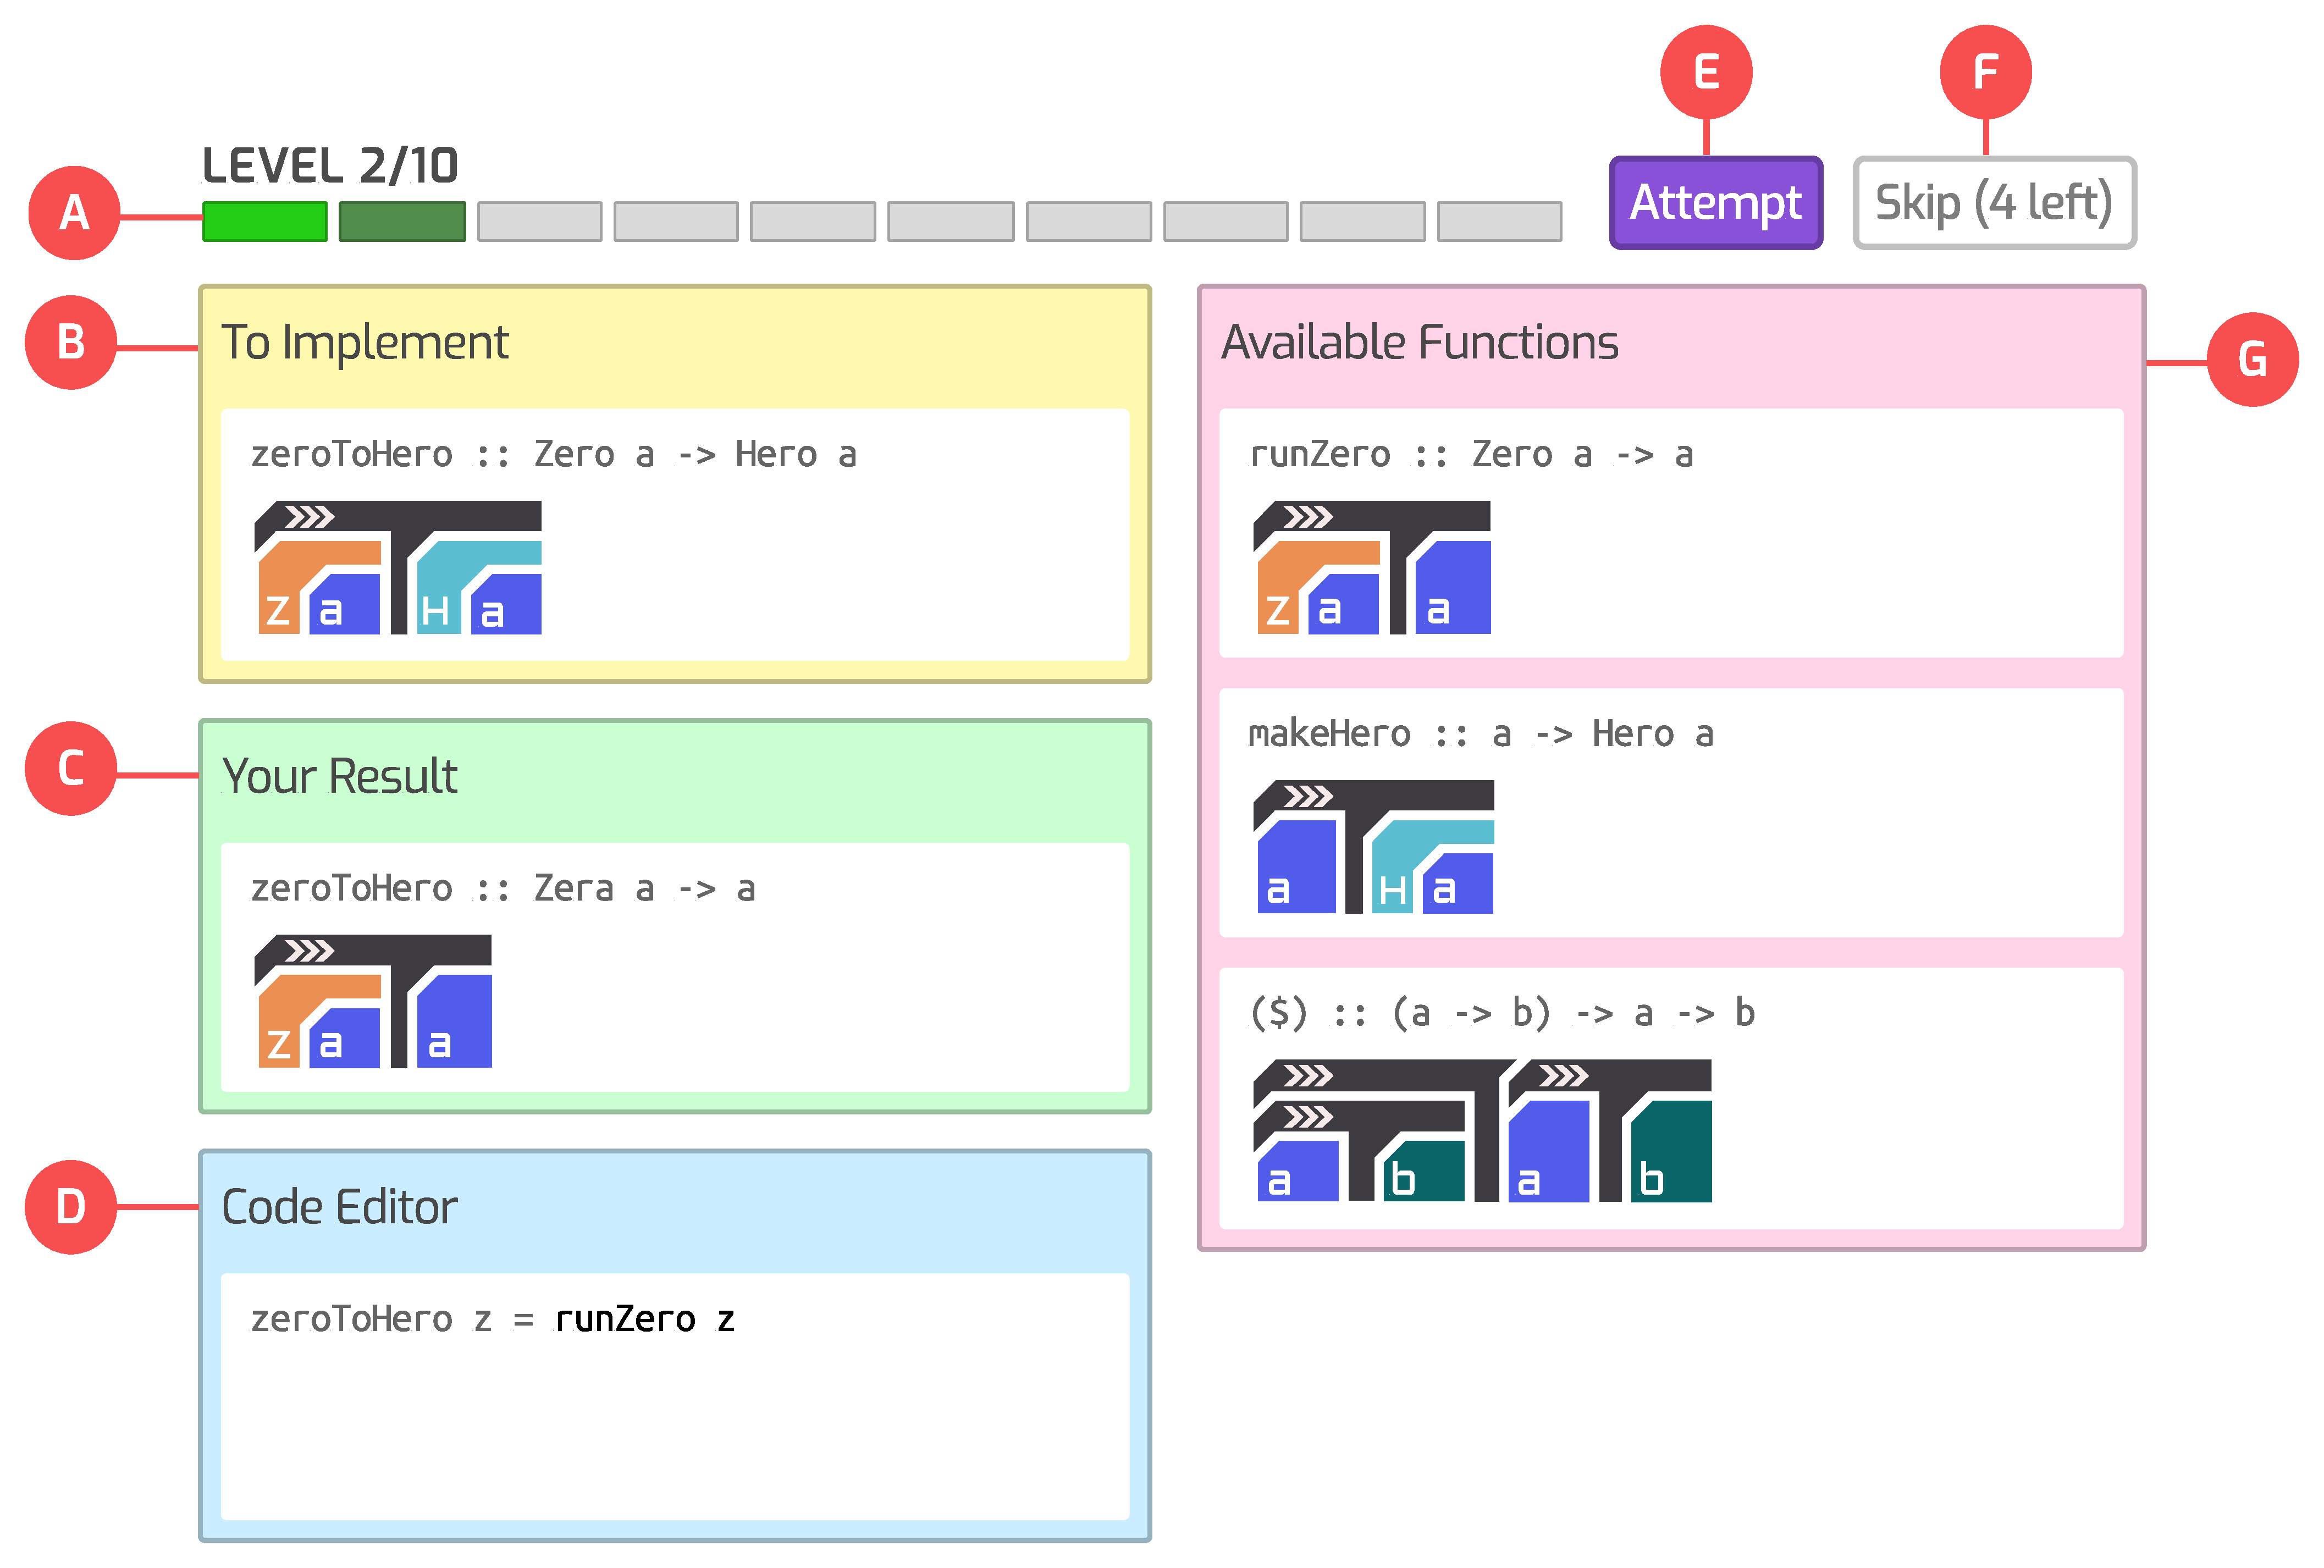
\includegraphics[width=\linewidth]{figures/Level2}
  \caption{\label{fig:level-example} A screenshot from the \DIFdelbeginFL \DIFdelFL{game ZeroToHero}\DIFdelendFL \DIFaddbeginFL \DIFaddFL{user study}\DIFaddendFL . \DIFdelbeginFL \DIFdelFL{On }\DIFdelendFL \DIFaddbeginFL \DIFaddFL{For }\DIFaddendFL this \DIFdelbeginFL \DIFdelFL{level }\DIFdelendFL \DIFaddbeginFL \DIFaddFL{task }\DIFaddendFL -- level 2 (Shown at A) -- the players need to implement the function \texttt{ zeroToHero :: Zero a -> Hero a} (B). They write their own definitions in the code editor (D) using a set of provided functions (G). The inferred type of their current definition is shown in (C). When ready, they can test their solution by clicking on the \textit{Attempt} button (E). They can also skip a level by clicking on the \textit{Skip (n left)} button next to it (F).}

\end{figure}

We illustrate the \DIFdelbegin \DIFdel{task }\DIFdelend \DIFaddbegin \DIFadd{tasks }\DIFaddend of the user study using levels 2 and 3 \DIFdelbegin \DIFdel{of the game. At }\DIFdelend \DIFaddbegin \DIFadd{as examples. For }\DIFaddend level 2 (Fig. \ref{fig:level-example}), the players need to implement the function \texttt{ zeroToHero :: Zero a -> Hero b}. The available functions are \texttt{runZero::Zero a -> a}, \texttt{makeHero:: a -> Hero a}. A generic function \texttt{(\$)} is provided to improve the ergonomics of composing functions, but all tasks can be completed without the use of generic functions. The possible \DIFdelbegin \DIFdel{solution }\DIFdelend \DIFaddbegin \DIFadd{solutions }\DIFaddend and other details of the level can be found in \DIFdelbegin \DIFdel{the appendix (Appendix \ref{levels})}\DIFdelend \DIFaddbegin \DIFadd{Appendix \ref{levels}}\DIFaddend . To complete this level, players only need to use each of the provided \DIFdelbegin \DIFdel{function once. The implementation }\DIFdelend \DIFaddbegin \DIFadd{functions once. One possible solution to this task would be }\DIFaddend {\tt zeroToHero z = makeHero (runZero z)}\DIFdelbegin \DIFdel{is one possible solution}\DIFdelend \DIFaddbegin \DIFadd{. The user illustrated in Fig. \ref{fig:level-example} did not reach a correct solution, as the type signature and GeckoGraph in }{\it \DIFadd{To Implement}} \DIFadd{panel do not match the one in }{\it \DIFadd{Your Result}} \DIFadd{panel}\DIFaddend .

\begin{figure}[!h]
  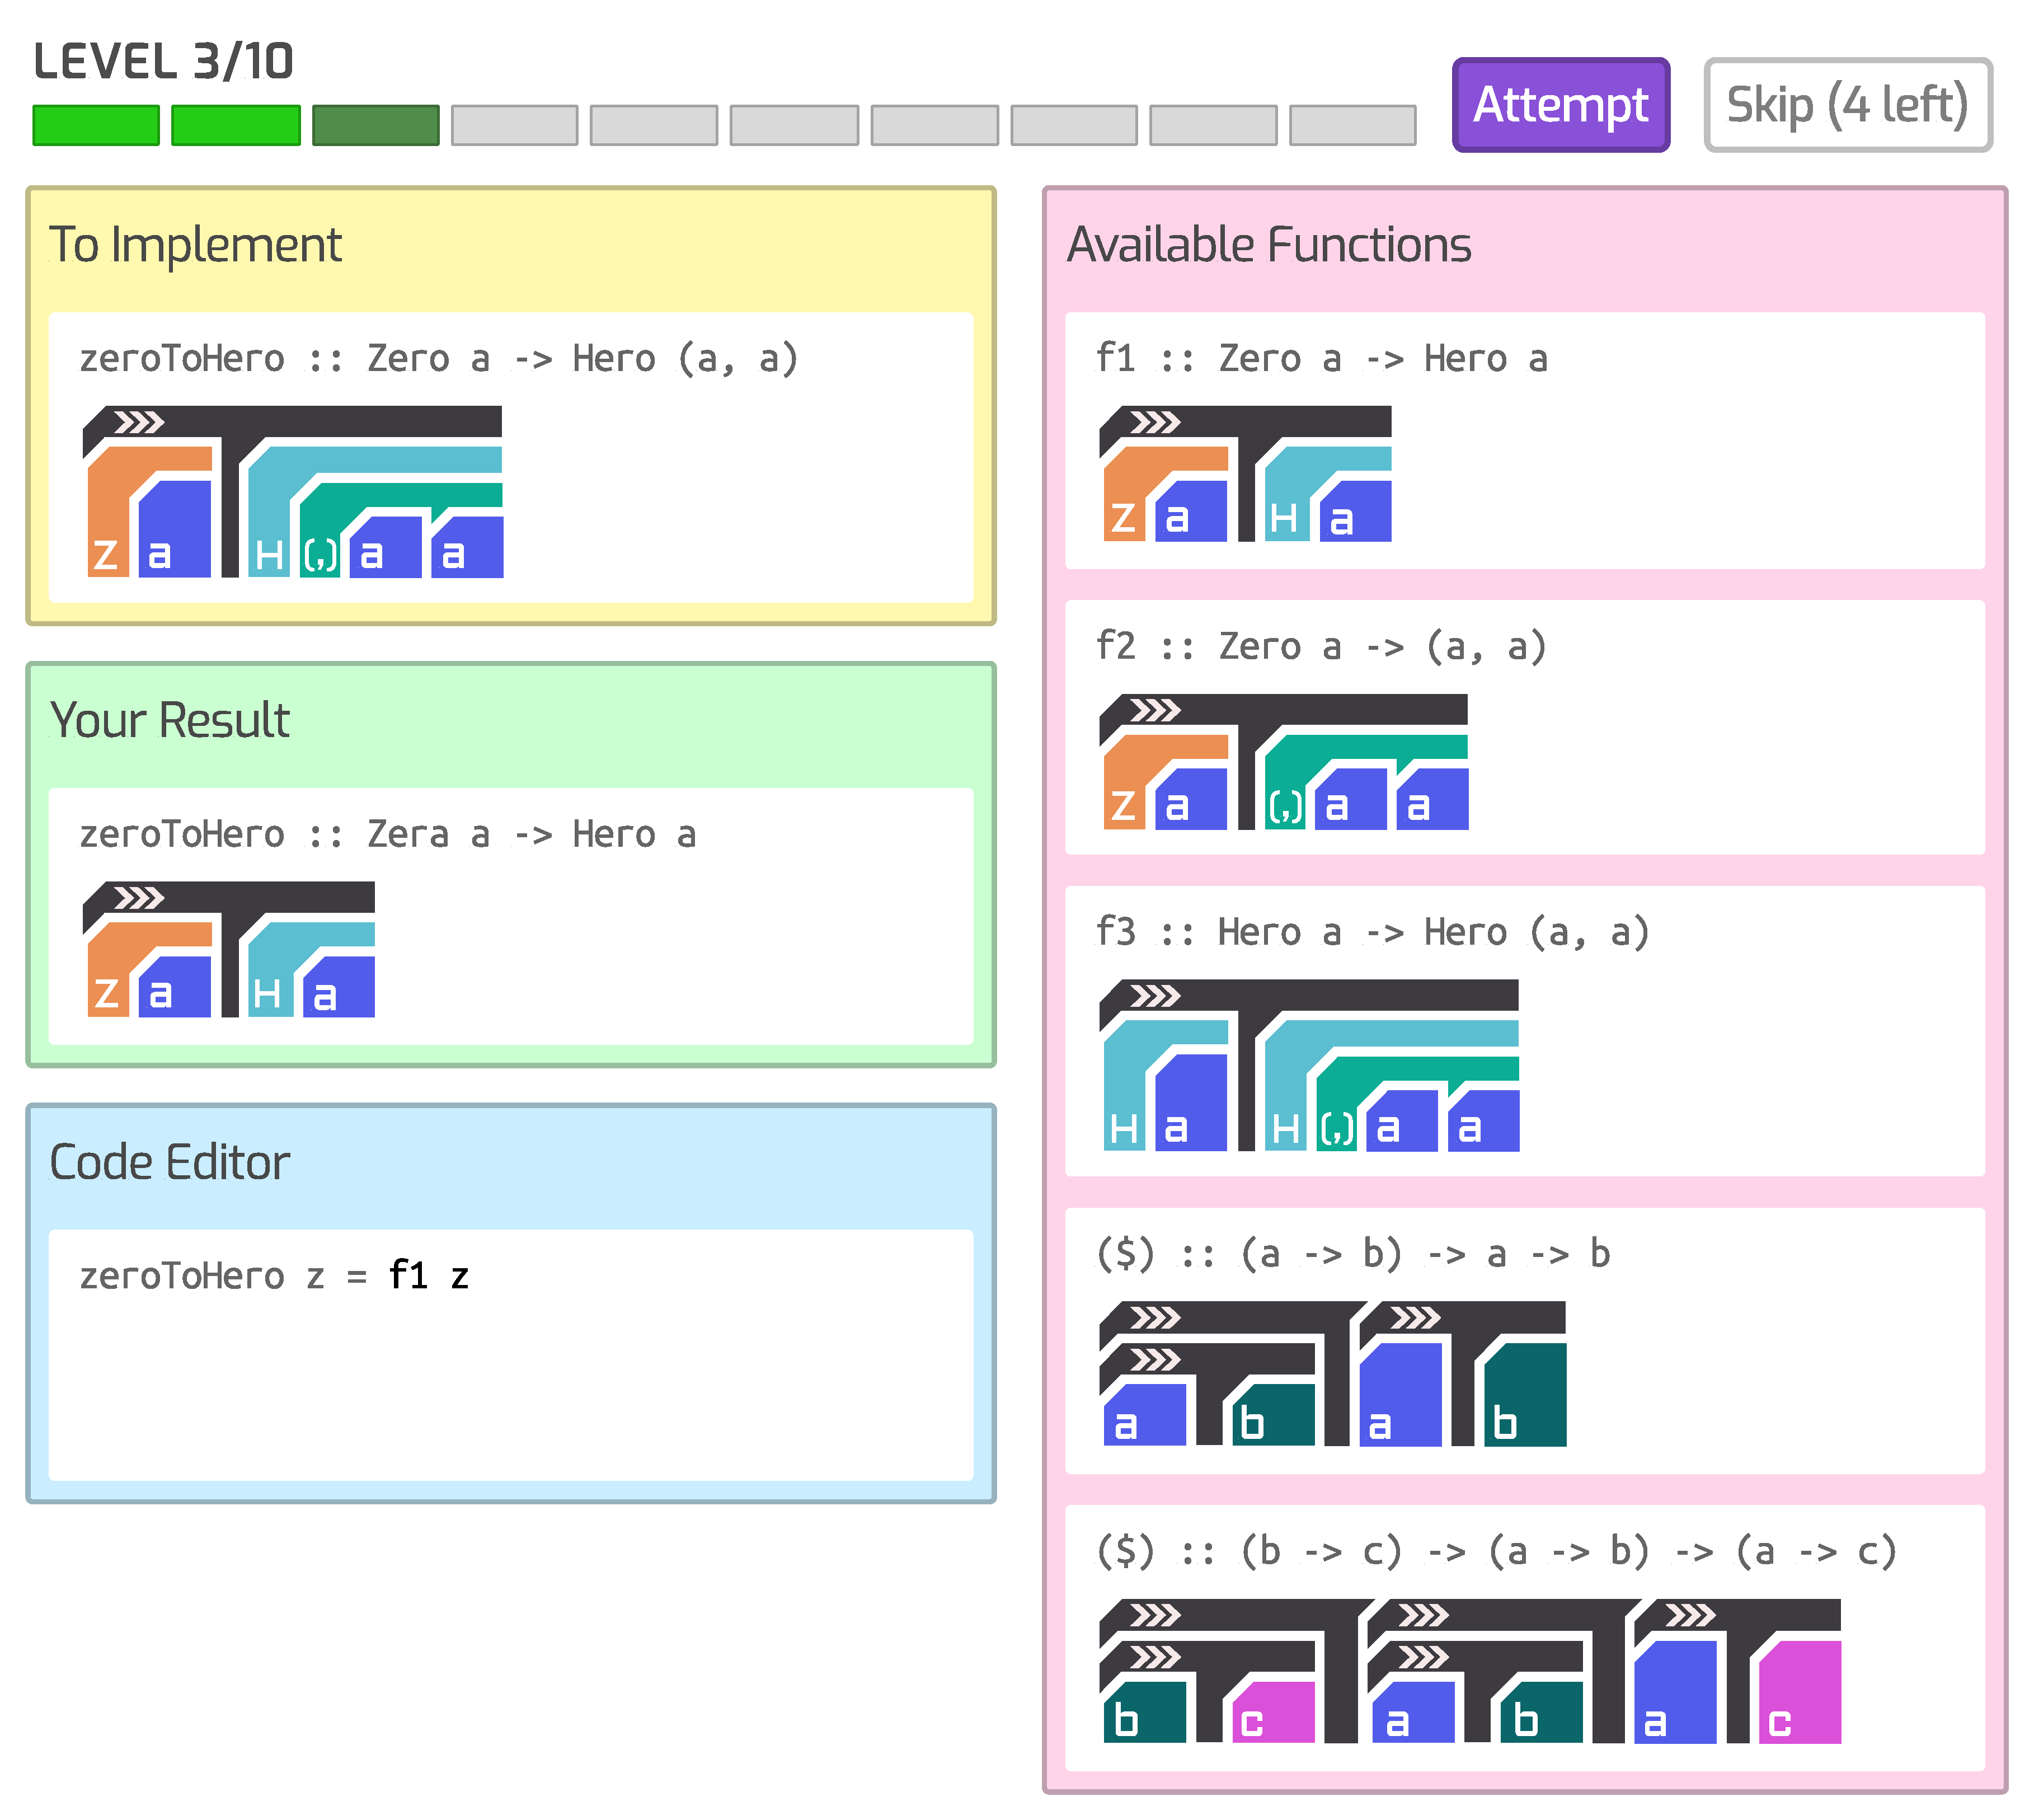
\includegraphics[width=\linewidth]{figures/Level3}
  \caption{\label{fig:level3} A screenshot showing \DIFdelbeginFL \DIFdelFL{the }\DIFdelendFL level 3 of the \DIFdelbeginFL \DIFdelFL{game ZeroToHero}\DIFdelendFL \DIFaddbeginFL \DIFaddFL{user study}\DIFaddendFL .  In this level, the players need to implement the function \texttt{ zeroToHero :: Zero a -> Hero (a a)}. Players are helped by the functions: {\tt f1 :: Zero a -> Hero a}, {\tt f2 :: Zero a -> (a, a)}, and {\tt f3 :: Hero a -> Hero (a, a)}.}
\end{figure}


In level 3 (Fig. \ref{fig:level3}),  players need to implement the function {\tt zeroToHero :: Zero a -> Hero (a, a)}.  In this level, not all provided functions are \DIFdelbegin \DIFdel{used in the final result}\DIFdelend \DIFaddbegin \DIFadd{useful}\DIFaddend . In particular,  players must discover that only \texttt{f1} and \texttt{f3} are necessary to produce the desired results. One implementation that satisfies the target type is \texttt{zeroTohero z = f3 (f1 z)}. Another possible implementation is {\tt zeroToHero z = f3 . f1 \$ z}, exercising the Haskell function composition idioms. \DIFaddbegin \DIFadd{Again, the user illustrated in Fig. \ref{fig:level3} did not reach a correct solution, as the type signature and GeckoGraphs in }{\it \DIFadd{To Implement}} \DIFadd{and }{\it \DIFadd{Your Result}} \DIFadd{do not match.
}\DIFaddend 


\subsection{Recruitment}
Participants were recruited online through the Haskell community on Reddit and Discord. Participation is fully anonymized; detailed ethical implications of these experiments were reviewed and approved by the IRB of the authors' institution.

\subsection{Group Assignments}

\DIFdelbegin \DIFdel{The experiment uses a between-subject design. }\DIFdelend Participants are assigned to one of two groups \DIFdelbegin \DIFdel{. The }\DIFdelend \DIFaddbegin \DIFadd{(A and B). The experiment uses between-subjects design \mbox{%DIFAUXCMD
\cite{Fisher1949-fn}}\hskip0pt%DIFAUXCMD
.  The }\DIFaddend tasks assigned to the two groups are \DIFdelbegin \DIFdel{in the sameorder. Participants }\DIFdelend \DIFaddbegin \DIFadd{the same. All participants }\DIFaddend receive both treatments (with and without GeckoGraph) during their runs\DIFaddbegin \DIFadd{, }\DIFaddend but in a different order.   \DIFdelbegin \DIFdel{Group one }\DIFdelend \DIFaddbegin {\bf \DIFadd{Group A}} \DIFaddend is assisted by GeckoGraph on even levels and \DIFdelbegin \DIFdel{text-only }\DIFdelend \DIFaddbegin \DIFadd{text-based }\DIFaddend type annotation on odd levels. \DIFdelbegin \DIFdel{Group two participants are the same but with the order flipped}\DIFdelend \DIFaddbegin {\it \DIFadd{Group B}} \DIFadd{is assisted by text-based type annotation on even levels and GeckoGraph on odd levels}\DIFaddend . The number of participants in the two groups is counterbalanced.

\subsection{Hypothesis}
In programming tasks that involve reading and understanding polymorphic types, graphic notation using visual elements that provide higher grouping strength (colors, shapes, sizes, and symbols) can improve the performance of such tasks compared to traditional text-based type notation. Our null hypothesis is: {\it Using graphic notation has no effect compared to traditional text-based type notation.} This hypothesis and the task design were registered at the Open Science Foundation prior to data collection \cite{Stuckey2023-vl}. 

\subsection{Task Design} \label{subsection:task}
During the study, participants \DIFdelbegin \DIFdel{receive }\DIFdelend \DIFaddbegin \DIFadd{received }\DIFaddend 10 tasks\DIFdelbegin \DIFdel{, represented by the 10 levels of the game }%DIFDELCMD < {\it %%%
\DIFdel{zeroToHero}%DIFDELCMD < }%%%
\DIFdelend . The tasks start off easy but gradually increase in difficulty.  In each task, a target type of the function \texttt{zeroToHero} is shown to the participants. Participants are provided with a list of available functions to implement the target function and to ensure it assumes the target type. This is to simulate the tasks of selecting useful functions from a library. Participants are not allowed to use any other functions or variables outside the provided functions; even the Haskell prelude is not available. This ensures that everyone has the same knowledge and minimizes the effect of familiarity. 

Participants can skip a level \DIFdelbegin \DIFdel{during the game }\DIFdelend if they are stuck. We believe that it is normal for anyone to get stuck on a challenging task, and being stuck on one of the 10 tasks does not discount their feedback \DIFdelbegin \DIFdel{of }\DIFdelend \DIFaddbegin \DIFadd{on }\DIFaddend the tool. \DIFdelbegin \DIFdel{We limit the }\DIFdelend \DIFaddbegin \DIFadd{The }\DIFaddend number of skips \DIFdelbegin \DIFdel{that }\DIFdelend a participant can use \DIFdelbegin \DIFdel{during the game to fourso that submitting }\DIFdelend \DIFaddbegin \DIFadd{is limited to four, so that it is not possible to submit }\DIFaddend qualitative feedback without completing at least \DIFdelbegin \DIFdel{some levels is impossible. 
}\DIFdelend \DIFaddbegin \DIFadd{6 tasks out of 10. 
}\DIFaddend 

\subsection{Measurements}
During the study, the time spent by participants on each task is recorded. We also record the resulting status of each level, whether it is a success or a failure. Before \DIFdelbegin \DIFdel{each run}\DIFdelend \DIFaddbegin \DIFadd{starting the study}\DIFaddend , participants nominate their level of Haskell experience on a four-level scale: beginner, familiar,  knowledgeable, and expert.  If a participant has completed all 10 levels (with the help of skipping), we invite the participant to complete a post-study survey. In it, we ask for \DIFdelbegin \DIFdel{their opinion on how intuitive }\DIFdelend \DIFaddbegin \DIFadd{them to rate how }{\bf \DIFadd{intuitive}} \DIFaddend the GeckoGraph design is, how \DIFdelbegin \DIFdel{distracting }\DIFdelend \DIFaddbegin {\bf \DIFadd{distracting}} \DIFaddend they find GeckoGraph, and how \DIFdelbegin \DIFdel{helpful GeckoGraph is during the game}\DIFdelend \DIFaddbegin {\bf \DIFadd{helpful}} \DIFadd{GeckoGraph is}\DIFaddend , using a seven-point scale. In the end, we ask \DIFdelbegin \DIFdel{a few }\DIFdelend \DIFaddbegin \DIFadd{2 }\DIFaddend open-ended questions\DIFdelbegin \DIFdel{, inviting participants to provide their }\DIFdelend \DIFaddbegin \DIFadd{: }{\it \DIFadd{What is your overall }\DIFaddend experience using GeckoGraph\DIFdelbegin \DIFdel{and their expectations about }\DIFdelend \DIFaddbegin } \DIFadd{and }{\it \DIFadd{What are your expectations on }\DIFaddend the potential applications of GeckoGraph\DIFaddbegin }\DIFaddend .

Data collection \DIFdelbegin \DIFdel{from }\DIFdelend \DIFaddbegin \DIFadd{of }\DIFaddend the study was stopped after the planned cut-off period of 14 days. After the cut-off date, the ZeroToHero \DIFdelbegin \DIFdel{game is open source }\DIFdelend \DIFaddbegin \DIFadd{website is open-sourced }\DIFaddend and available for free evaluation\footnote{https://zerotohero.fly.dev}\DIFaddbegin \DIFadd{, }\DIFaddend and repeating our experiment\DIFdelbegin \DIFdel{, but }\DIFdelend \DIFaddbegin \DIFadd{. However, }\DIFaddend no further data was collected. 

\section{Results} \DIFaddbegin \label{sec:results}
\DIFaddend 

During the data collection period, a total of 714 users participated in the study. Among them, 245 are novice users, 216 are familiar with Haskell, 216 are knowledgeable users, and 88 are expert users. 

\subsection{Time to complete levels}

The 10 levels are designed to increase difficulty gradually. From the results of the experiment, most of the tasks align with this trend. However, three tasks stand out in Fig. \ref{fig:level-time}.  Level 7 (mean = 334 seconds) is the hardest task in \DIFdelbegin \DIFdel{the game in }\DIFdelend terms of time, followed by level 8 (mean = 228 seconds) and level 5 (mean = 224 seconds). To complete an average level, the beginner group uses an average of 100 seconds, the familiar group uses 90 seconds, the knowledgeable group uses 80 seconds, and the expert group uses 70 seconds. This roughly aligns with self-reported expertise. We show that the task time on each level follows normal distributions using a Shapiro-Wilk test \cite{Shaphiro1965-dx} (p-value  $ \leq 1.018 \times 10^-16$, for an alpha value of 0.05, p less than 0.05 is considered \DIFaddbegin \DIFadd{a }\DIFaddend normal distribution).

Levels 5, 7, and 8 are the only three levels that include functions from \DIFaddbegin \DIFadd{the }\DIFaddend standard Haskell library \DIFdelbegin \DIFdel{, baring the }\DIFdelend \DIFaddbegin \DIFadd{other than the generic }\DIFaddend \texttt{(.)} and \texttt{(\$)}\DIFdelbegin \DIFdel{provided for }\DIFdelend \DIFaddbegin \DIFadd{, which are provided for pure }\DIFaddend convenience. Level 5 requires programmers to use the \texttt{fst} and \texttt{snd} functions to extract \DIFaddbegin \DIFadd{a }\DIFaddend value from a tuple. Level 7 requires programmers to use the \texttt{(<*>)} function of the \texttt{Applicative} class, while level 8 requires the \texttt{fmap} function of the \texttt{Functor} class. The authors speculate that the more experienced participants are much more familiar with these functions, hence the strong contrast on these three levels. 

However, when comparing the task time between the two treatments, we were unable to reject the null hypothesis. In a two-sample T-test, we could not find any significant difference between the two groups overall (p-value = 0.457), nor \DIFdelbegin \DIFdel{does }\DIFdelend \DIFaddbegin \DIFadd{did }\DIFaddend there differ between the two groups in any of the four levels of experience (beginner: p-value = 0.845, familiar: p-value = 0.524, Knowledgeable: p-value = 0.712, expert\DIFaddbegin \DIFadd{: }\DIFaddend p-value = 0.771).

\begin{figure}[]
  \includegraphics[width=\linewidth]{figures/LevelTime}
  \caption{\label{fig:level-time} Time spent on each level, with 95\% confidence interval. We show that the difficulty steadily increases across the \DIFdelbeginFL \DIFdelFL{game}\DIFdelendFL \DIFaddbeginFL \DIFaddFL{user study}\DIFaddendFL , but levels 5, 7, and 8 are significantly harder than the authors intended. The overall task time of each group roughly matches \DIFaddbeginFL \DIFaddFL{the }\DIFaddendFL experience level.}
\end{figure}

\subsection{Success rate}
We saw that, overall, GeckoGraph provides a \DIFaddbegin \DIFadd{slightly }\DIFaddend higher success rate (96.88\%) than text-based type notation (94.62\%). This trend can be seen in every experienced group: beginner group (\DIFdelbegin \DIFdel{95. 12}\DIFdelend \DIFaddbegin \DIFadd{95.12}\DIFaddend \% vs. \DIFdelbegin \DIFdel{92. 68}\DIFdelend \DIFaddbegin \DIFadd{92.68}\DIFaddend \%), familiar group (\DIFdelbegin \DIFdel{97. 39}\DIFdelend \DIFaddbegin \DIFadd{97.39}\DIFaddend \% vs. \DIFdelbegin \DIFdel{93. 34}\DIFdelend \DIFaddbegin \DIFadd{93.34}\DIFaddend \%), knowledgeable group (\DIFdelbegin \DIFdel{96. 82\% vs. 96. 06}\DIFdelend \DIFaddbegin \DIFadd{96.82\% vs.96.06}\DIFaddend \%), and expert group (\DIFdelbegin \DIFdel{98. 2\% vs. 96. 40}\DIFdelend \DIFaddbegin \DIFadd{98.2\% vs.96.40}\DIFaddend \%). We saw the significance decrease as the user's experience increased. When performing a proportion test on each group, we see that the effect is most significant with the beginner group and reject the null hypothesis (z score = 2.0228, p-value = 0.0431), followed by the familiar group (z score = 1.7495, p-value = 0.0802). The knowledgeable group (z score = 1.0295, p-value = 0.3032) and the expert group (z score = 0.8660, p-value = 0.3756) show less significant differences between treatments. 

When breaking down the result in each task (Fig. \ref{fig:success-rate}), we were able to reject the null hypothesis in task 10 of the beginner group \DIFdelbegin \DIFdel{and }\DIFdelend \DIFaddbegin \DIFadd{(94.9\% with GecoGraph, and 80.4\% without GeckoGraph, p-value=0.0452) and }\DIFaddend task 10 of the familiar group \DIFdelbegin \DIFdel{\ref{fig:success-rate}. 
We will address this correlation in Section~\ref{sec:discussion}.
}\DIFdelend \DIFaddbegin \DIFadd{(98.5\% with GecoGraph, and 87.3\% without GeckoGraph, p-value = 0.136). 
}\DIFaddend 

Level 10 is the most cognitively demanding: the provided functions are the lengthiest, and the solution is challenging and deceptive. Programmers must use the provided rotate function {\it f2} to adjust the positions of the four components of the {\it Zero} value four times to get to the correct position. Completing the level requires applying the functions {\it f1}, {\it f2}, and {\it f3} in a nested sequence that is 8 layers deep. Consequently, programmers need to frequently switch contexts to recall the purpose of each function. We speculate that this level demands the mental flexibility typical of a Haskell expert to internalize these functions quickly. GeckoGraph helps less experienced programmers to achieve the same level of comprehension fluency by adding \DIFdelbegin \DIFdel{structural }\DIFdelend \DIFaddbegin \DIFadd{visual }\DIFaddend clarity.

\begin{figure}[ht]
  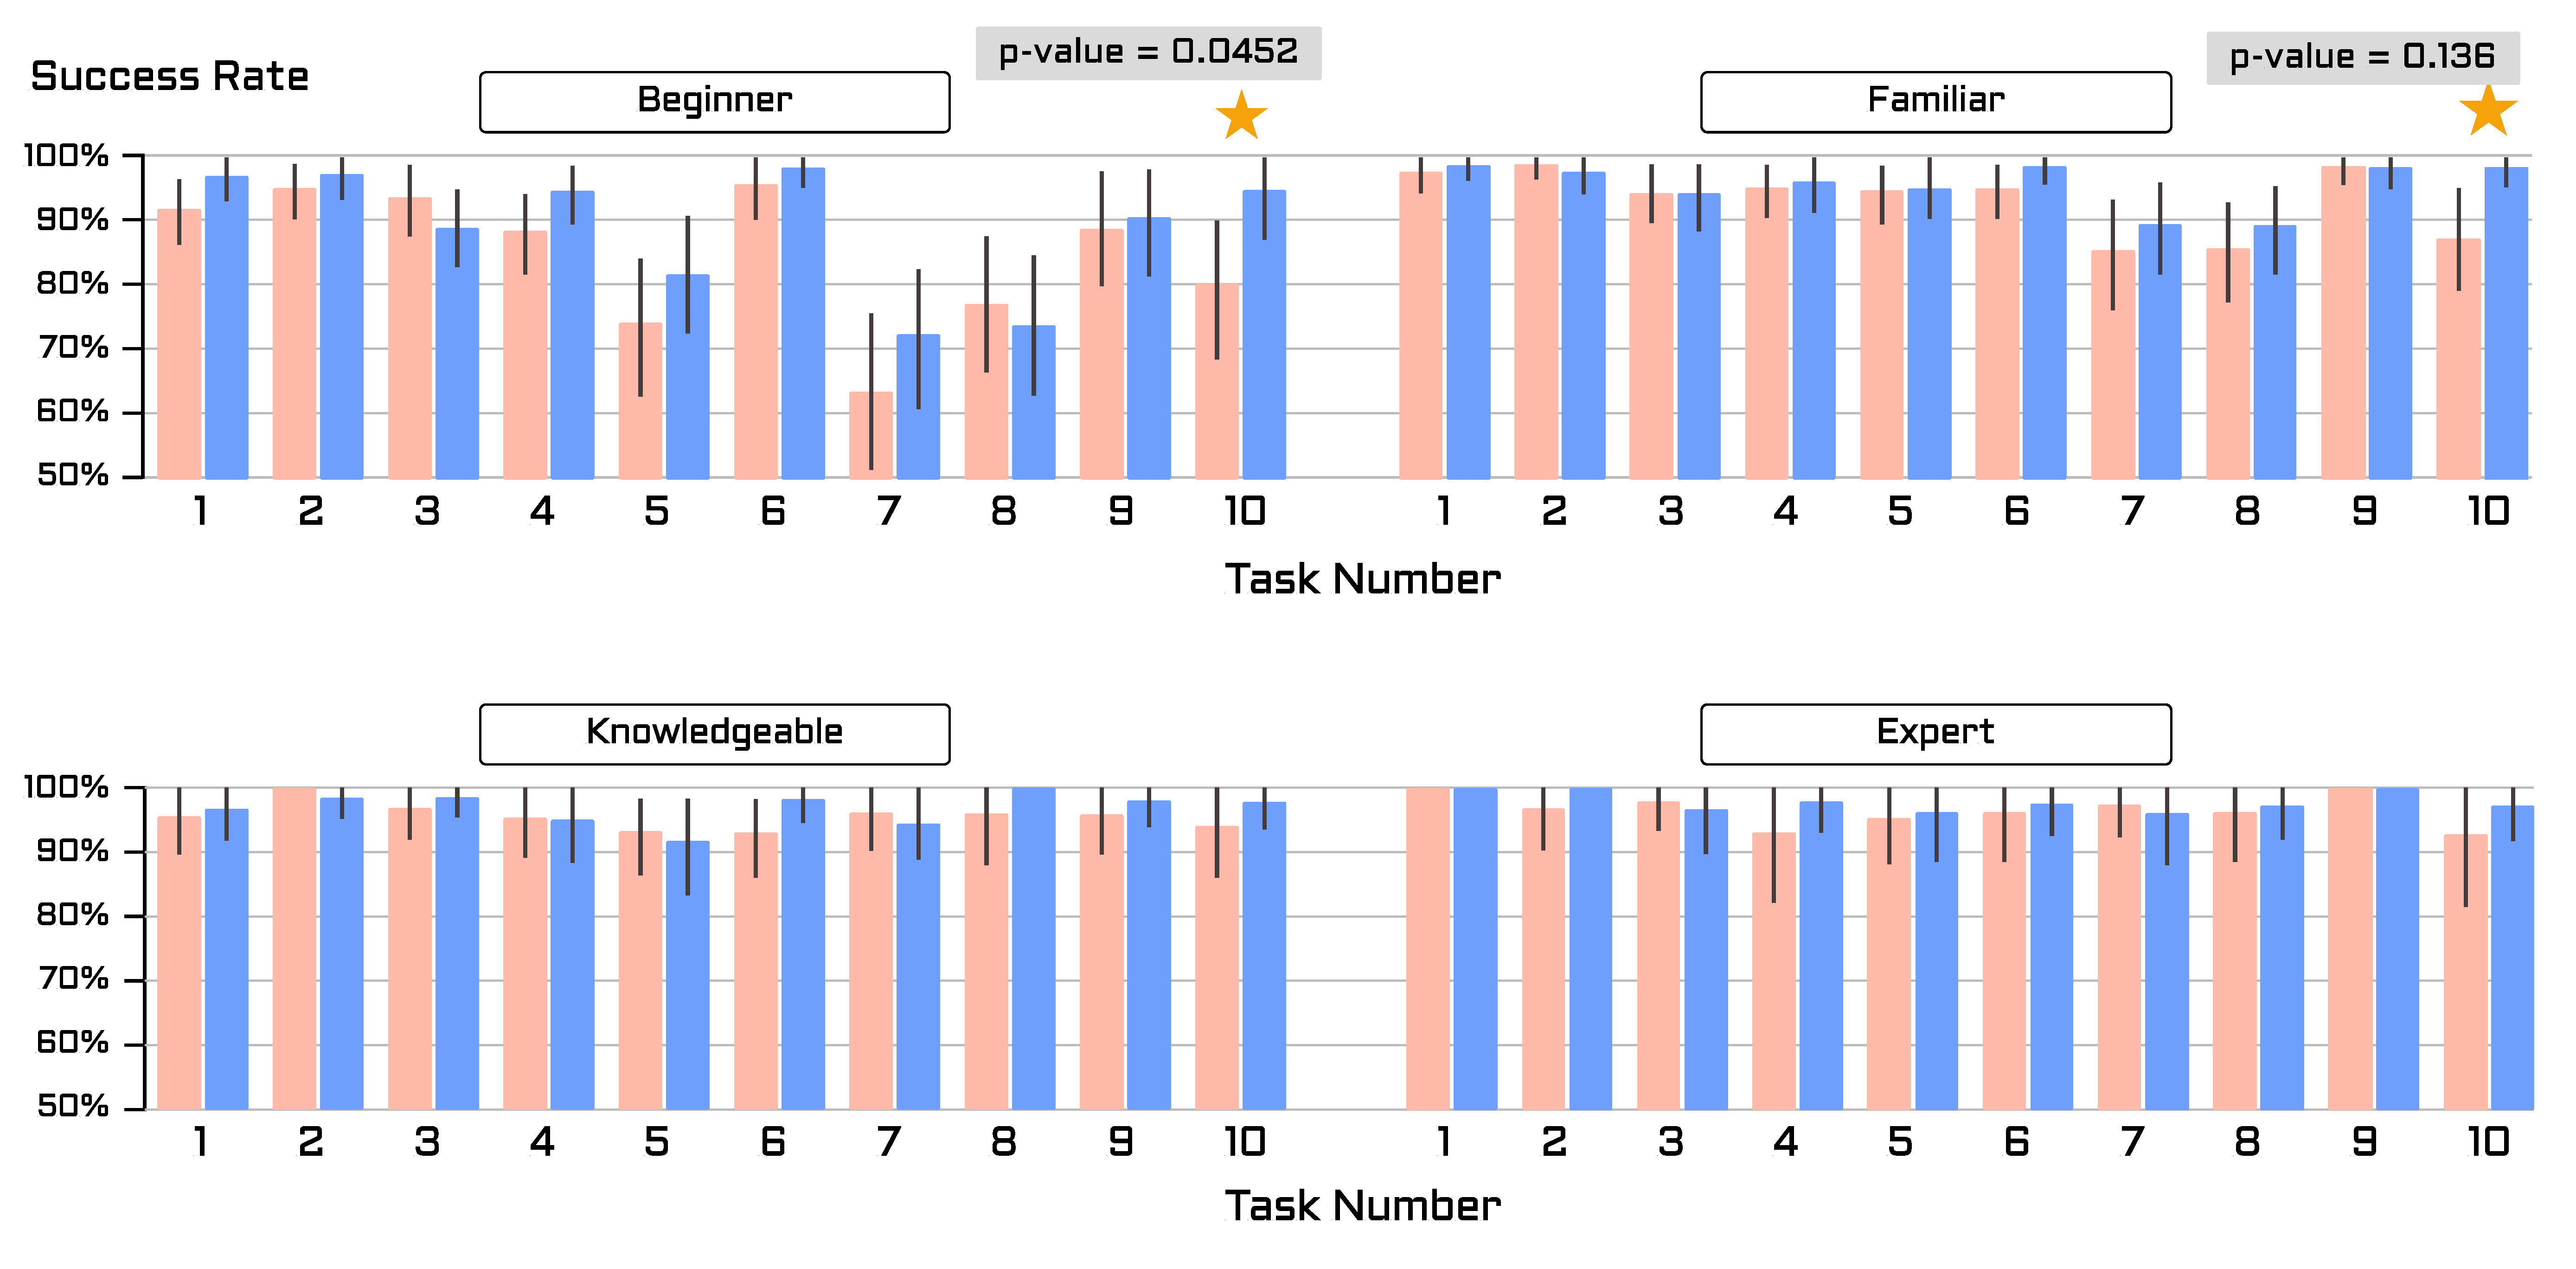
\includegraphics[width=\linewidth]{figures/SuccessfulRate}
  \caption{\label{fig:success-rate}{\bf Success rate of each task, with 95\% confidence interval, grouped by experience level.} The figure is cropped from 50\% to 100\% for readability. Bootstrapping was used for computing the confidence interval because of the non-normal distribution. In most tasks, GeckoGraph provides a small edge. However, significant differences were found in task 10 of the beginner group and task 10 of the familiar group. }
\end{figure}

\subsection{Qualitative Feedback}
In their responses to the post-study survey, \DIFdelbegin \DIFdel{most programmers believe that the design of GeckoGraph is intuitive }\DIFdelend \DIFaddbegin \DIFadd{participants showed mostly neutral sentiments towards GeckoGraph's design and appeal. They find GeckoGraph moderately intuitive to use }\DIFaddend and that its appearance in the interface does not cause distraction.
\DIFaddbegin 

\DIFaddend For the question ``Do you find the GeckoGraph distracting", most of the participants rated a \DIFdelbegin \DIFdel{negative }\DIFdelend \DIFaddbegin \DIFadd{low }\DIFaddend score, with an average of 2.88 (Fig. \ref{fig:qualitative} left). For the question ``How intuitive do you find the GeckoGraph?", we saw a reverse correlation of experience (Fig. \ref{fig:qualitative} Middle): experts find the GeckoGraph most intuitive (5.07), followed by the knowledgeable group (4.87), and the familiar group (4.80). The beginner group found it to be the least intuitive but still rated \DIFdelbegin \DIFdel{a positive }\DIFdelend \DIFaddbegin \DIFadd{it positively, albeit with a low }\DIFaddend score of 4.71. 
When answering the question ``How helpful do you find GeckoGraph in finding the solution\DIFdelbegin \DIFdel{during the game}\DIFdelend ?", the answer is more divided into different experience groups (Fig. \ref{fig:qualitative} right). It is slightly positive for beginners (\DIFaddbegin \DIFadd{mean=}\DIFaddend 4.25) and slightly negative for the other groups, the familiar group (\DIFaddbegin \DIFadd{mean=}\DIFaddend 3.86) and the knowledgeable group (\DIFaddbegin \DIFadd{mean=}\DIFaddend 3.32). The expert group finds that GeckoGraph is \DIFdelbegin \DIFdel{relatively unhelpful , with an average score of }\DIFdelend \DIFaddbegin \DIFadd{moderately unhelpful (mean=}\DIFaddend 2.95\DIFdelbegin \DIFdel{.
}\DIFdelend \DIFaddbegin \DIFadd{)
}\DIFaddend 

Two interesting trends emerge. First, \DIFdelbegin \DIFdel{the more experienced the users are , the more likely they are }\DIFdelend \DIFaddbegin \DIFadd{experienced users are more likely }\DIFaddend to find GeckoGraph intuitive and easy to use. This aligns with our design decision to make GeckoGraph resemble text-based type annotation. Those familiar with text-based type annotation find GeckoGraph second nature to read. Second, the correlation reverses when it comes to perceived helpfulness. The more experienced the users are, the less likely they are to find GeckoGraph helpful. We speculate this pattern occurs because users who are experts in text-based type annotations naturally prefer reading text-based notation and tend to ignore GeckoGraph, diminishing its usefulness. Conversely, novice users are more likely to be drawn to GeckoGraph and find that its visualization offers more clarity and useful insights.


% To quote some feedback from participants: ``Types are much easier to understand by the GeckoGraph than by trying to parse all parentheses and understand the types from the signature. " ``It makes it easier to see at a glance when your output type is correct or what the difference between the current type and the target is."

% To quote a participant, ``GeckoGraph is quite intuitive to see the permutations of the arguments. Also, to see how to produce and consume arguments." 

\begin{figure}[]
  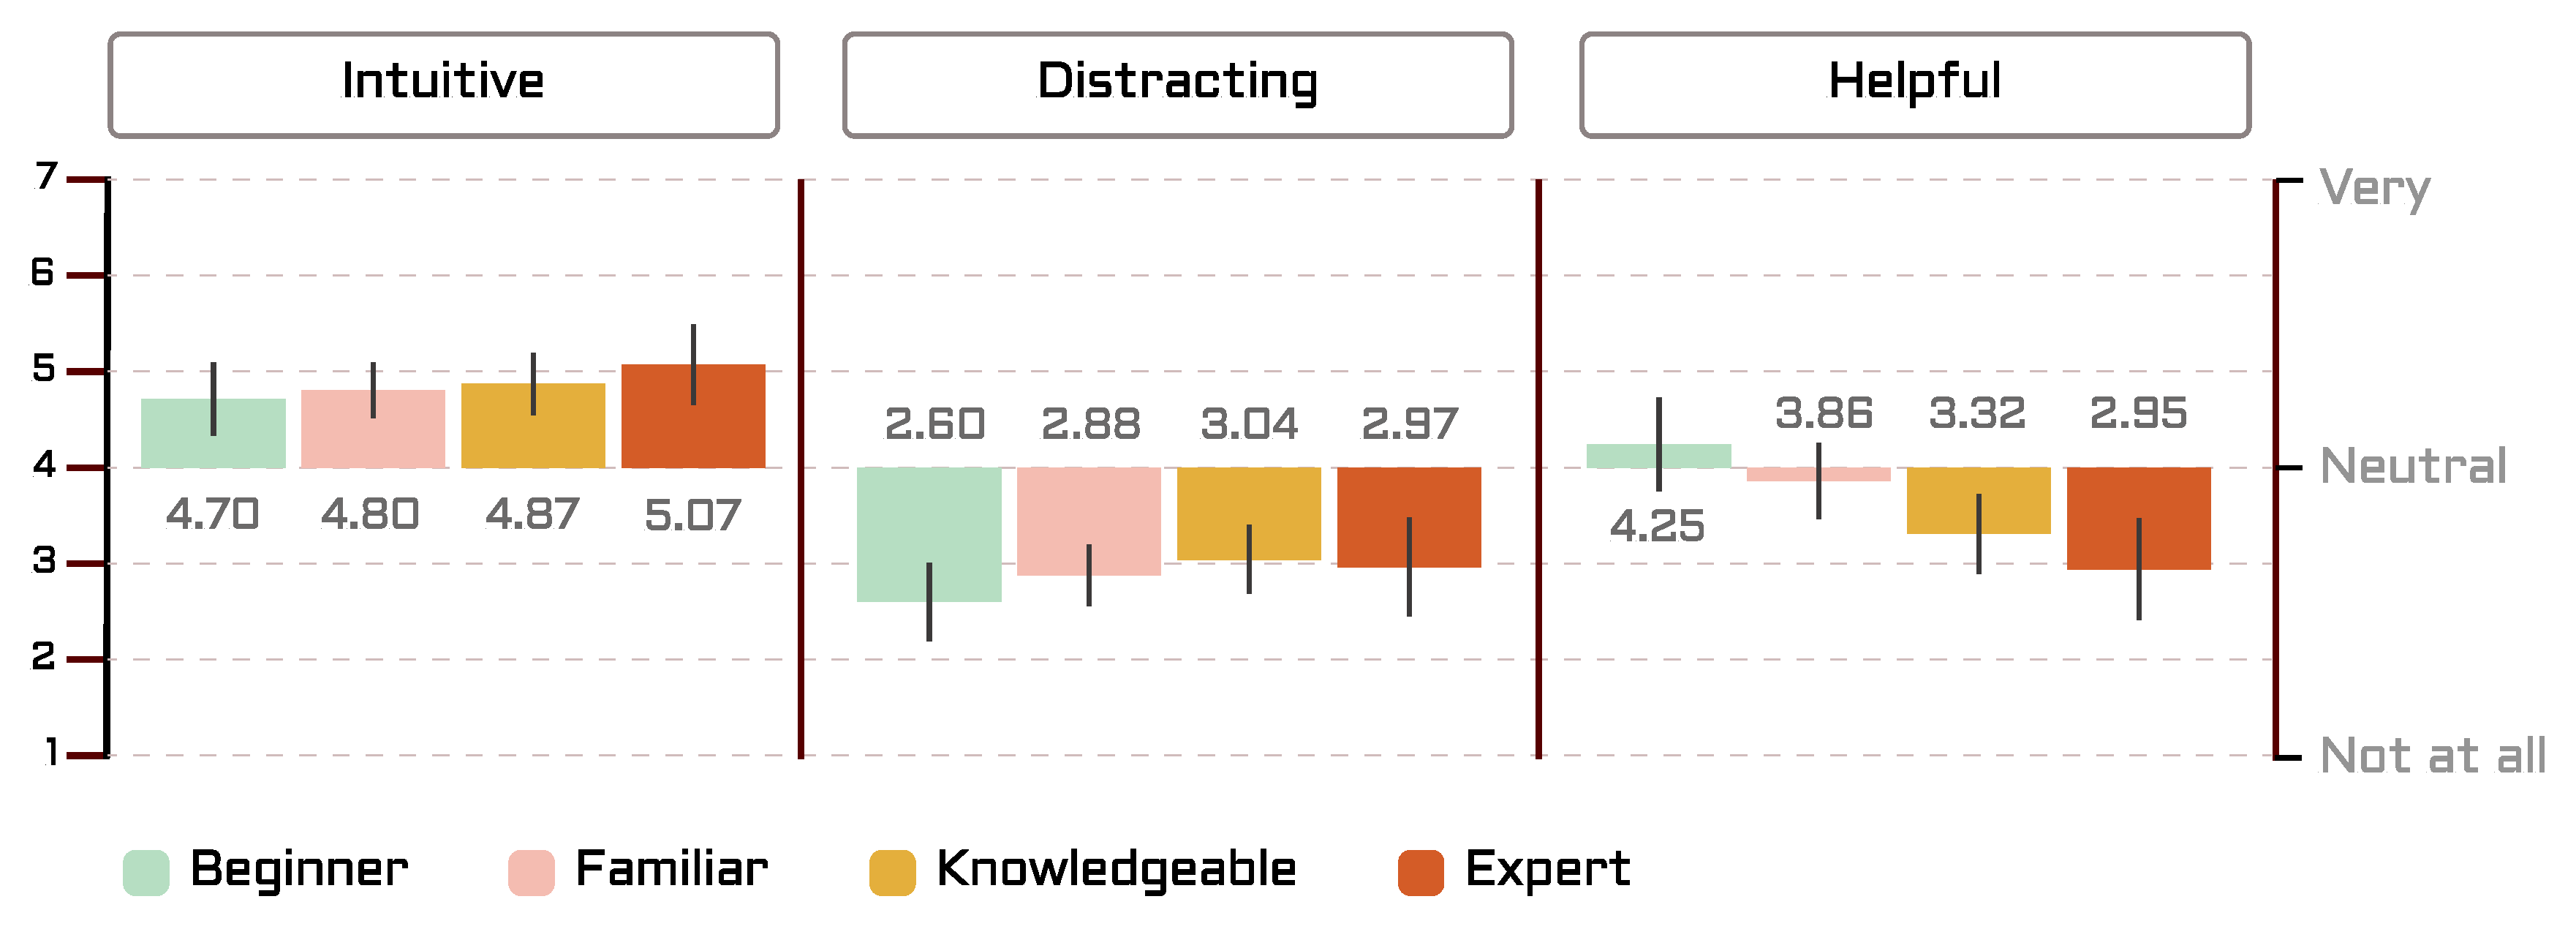
\includegraphics[width=\linewidth]{figures/Qualitative}
  \caption{\label{fig:qualitative} {\bf The users rated scores of how intuitive (left), distracting (middle), and helpful (right) they found GeckoGraph, with 95\% confidence interval.} Overall, programmers \DIFdelbeginFL \DIFdelFL{consider }\DIFdelendFL \DIFaddbeginFL \DIFaddFL{are neutral to }\DIFaddendFL GeckoGraph\DIFaddbeginFL \DIFaddFL{'s design. Some find GeckoGraph }\DIFaddendFL to be intuitive and not distracting. However, beginners are more likely than experienced functional programmers to find it helpful. }
\end{figure}

\subsection{Threats to validity}

\paragraph{Task design}
In our \DIFdelbegin \DIFdel{human }\DIFdelend \DIFaddbegin \DIFadd{user }\DIFaddend study, most of the provided functions are very abstract. These functions are created by the authors solely for the gamified study. They are designed to be different from well-known Haskell functions to minimize the familiarity variable. They are also designed with an interest in being challenging and fun. These functions may not be the most representative of real-world Haskell programming. 

\paragraph{The use of skips}
Although we justified the use of skips in Section \ref{subsection:task}, the availability of skipping does allow users to adopt more utilitarian strategies, often involving skipping a level without giving it a fair try. This happened more often in the later levels when users realized they had enough skip opportunities left to ``complete the game". These strategies may result in lower recorded success rates than if no skips were allowed.


\section{Discussion} \label{sec:discussion}
\DIFaddbegin 

\DIFadd{This section discusses the main findings and implications of our study. 
We speculate the strengths of GeckoGraph observed from both quantitative and qualitative results (Section~\ref{sec:discussion:strengths}). 
We then discuss the limitations of the current design (Section~\ref{sec:discussion:weaknesses}) and reflect on the gamified nature of our user study (Section~\ref{sec:discussion:gamification}). 
Finally, we identify potential applications of GeckoGraph in programming tools, documentation, and education (Section~\ref{sec:discussion:applications}).
}

\DIFaddend \subsection{Strengths}\DIFdelbegin \DIFdel{From the results of our experiment, we see }\DIFdelend \DIFaddbegin \label{sec:discussion:strengths}
\DIFadd{Overall, our experimental results show no statistically significant difference in task completion time between conditions with and without GeckoGraph. However, we find }\DIFaddend that using GeckoGraph \DIFdelbegin \DIFdel{has a significanteffect on the success rate of our participants, especially for less experienced programmers. We also see that with the data we collected, we did not find a significant time difference between programming with and without GeckoGraph . To extrapolate the observed expressiveness, we speculate on }\DIFdelend \DIFaddbegin \DIFadd{shows a significant, albeit moderate, effect on task success rates for beginners. In particular, on the hardest task (task 10), GeckoGraph improved the success rates across the two less experienced user groups by 14.5\% and 11.2\%, respectively. 
To interpret the observed advantages, we hypothesize }\DIFaddend the practical benefits \DIFdelbegin \DIFdel{of programming with GeckoGraph }\DIFdelend \DIFaddbegin \DIFadd{that GeckoGraph offers to programmers}\DIFaddend .

\subsubsection{\DIFdelbegin \DIFdel{Identify }\DIFdelend \DIFaddbegin \DIFadd{Identifying }\DIFaddend the Most Important Features}
\DIFdelbegin \DIFdel{One trend we saw from the qualitative feedback is that programmers find GeckoGraph }\DIFdelend \DIFaddbegin \DIFadd{Qualitative feedback revealed that programmers found GeckoGraph particularly }\DIFaddend helpful for spotting patterns and \DIFdelbegin \DIFdel{important features from the types. 
Programmers are very positive about GeckoGraph 's ability to reveal the most helpful features }\DIFdelend \DIFaddbegin \DIFadd{identifying important features in type signatures. 
Participants appreciated how GeckoGraph highlights key aspects }\DIFaddend of a type \DIFdelbegin \DIFdel{in distinctive visual elements }\DIFdelend \DIFaddbegin \DIFadd{using distinctive visual properties }\DIFaddend such as color, length, and height. 
\DIFdelbegin \DIFdel{To quote some feedback from participants}\DIFdelend \DIFaddbegin \DIFadd{Representative comments include}\DIFaddend : 
``{\it Types are much easier to understand \DIFdelbegin \DIFdel{by the }\DIFdelend \DIFaddbegin \DIFadd{with }\DIFaddend GeckoGraph than by trying to parse all parentheses and understand the types from the signature.}\DIFdelbegin \DIFdel{" }\DIFdelend \DIFaddbegin \DIFadd{'' and 
}\DIFaddend ``{\it It makes it easier to see at a glance when your output type is correct or what the difference between the current type and the target is.}\DIFdelbegin \DIFdel{"
}\DIFdelend \DIFaddbegin \DIFadd{''
}\DIFaddend 

\subsubsection{\DIFdelbegin \DIFdel{Generalize patterns }\DIFdelend \DIFaddbegin \DIFadd{Generalizing Patterns }\DIFaddend in \DIFdelbegin \DIFdel{type classes}\DIFdelend \DIFaddbegin \DIFadd{Type Classes}\DIFaddend }
A common source of confusion among novice Haskell programmers is distinguishing between functions that operate on \DIFdelbegin \DIFdel{generalized }\DIFdelend \DIFaddbegin \DIFadd{generic }\DIFaddend types and those that work \DIFdelbegin \DIFdel{with }\DIFdelend \DIFaddbegin \DIFadd{on }\DIFaddend concrete types \cite{Tirronen2015-nr}. 
For \DIFdelbegin \DIFdel{instance, the type constraints }\DIFdelend \DIFaddbegin \DIFadd{example, differentiating between }\DIFaddend {\tt Integral a => a} and {\tt Integer}, {\tt Floating a => a} and {\tt Float}, \DIFdelbegin \DIFdel{as well as }\DIFdelend \DIFaddbegin \DIFadd{or }\DIFaddend {\tt Foldable} \DIFdelbegin \DIFdel{instances versus }\DIFdelend \DIFaddbegin \DIFadd{and }\DIFaddend {\tt []} can be \DIFdelbegin \DIFdel{particularly challenging. 
Many Haskell learners may find the differences between concrete types and their generic counterparts }\DIFdelend \DIFaddbegin \DIFadd{difficult. 
Learners often find such distinctions }\DIFaddend irrelevant to their \DIFdelbegin \DIFdel{programming tasks, thereby complicating their quest for solutions.
In the example }\DIFdelend \DIFaddbegin \DIFadd{immediate tasks, which complicates problem-solving and error interpretation.
}

\DIFadd{As }\DIFaddend shown in Fig.\DIFdelbegin \DIFdel{\ref{fig:example-foldable}, }\DIFdelend \DIFaddbegin \DIFadd{~\ref{fig:example-foldable}, when }\DIFaddend a programmer mistakenly supplies a \texttt{Char} instead of a \texttt{String}\DIFdelbegin \DIFdel{literal. The compiler responds with an error message that compares the provided }\texttt{\DIFdel{Char}} %DIFAUXCMD
\DIFdel{type to a confusingly named }\DIFdelend \DIFaddbegin \DIFadd{, the compiler reports a confusing mismatch involving a generalized }\DIFaddend type \texttt{t0 a0}. 
In \DIFdelbegin \DIFdel{this case, the information has been generalized too much and the programmer can hardly find their bearing to the original problem. This level of generalization can undermine a programmer's confidence in understanding the language and navigating type errors. In }\DIFdelend GeckoGraph, both list types and types with a \DIFdelbegin \DIFdel{Foldable instance share a similar structure. 
Therefore, the type }\texttt{\DIFdel{t0 a0}} %DIFAUXCMD
\DIFdel{in the error message matches the shape of }\texttt{%DIFDELCMD < [%%%
\DIFdel{a}%DIFDELCMD < ]%%%
}%DIFAUXCMD
\DIFdel{. Bring the programmer closer to the real issue, trying to match a complex type with a concrete simple type. This feature lowers the entry barrier for languages like }\DIFdelend \DIFaddbegin \texttt{\DIFadd{Foldable}} \DIFadd{instance share similar visual structures. 
This correspondence helps programmers relate generalized types back to familiar concrete ones, lowering the cognitive barrier to understanding polymorphism. 
Such visual consistency is especially valuable in }\DIFaddend Haskell, where even \DIFdelbegin \DIFdel{basic arithmetic functions }\DIFdelend \DIFaddbegin \DIFadd{simple arithmetic operators like }\DIFaddend {\tt +} and {\tt -} are defined \DIFdelbegin \DIFdel{on generic types.
This approach lowers the barrier to introducing foundational language concepts without sacrificing generality.
}\DIFdelend \DIFaddbegin \DIFadd{generically.
}\DIFaddend 

\subsubsection{Consistent \DIFdelbegin \DIFdel{color scheme}\DIFdelend \DIFaddbegin \DIFadd{Color Scheme}\DIFaddend }\label{par:color-scheme}
A \DIFdelbegin \DIFdel{common }\DIFdelend \DIFaddbegin \DIFadd{frequent }\DIFaddend task in programming is \DIFdelbegin \DIFdel{to scan for }\DIFdelend \DIFaddbegin \DIFadd{scanning through documentation or libraries to find }\DIFaddend a desired function\DIFdelbegin \DIFdel{from a sea of potentially useful functions, such as library documentation. During scanning, programmers often have partial knowledge of the desired function, e.g., the arity, one of the }\DIFdelend \DIFaddbegin \DIFadd{, often based on partial knowledge such as }\DIFaddend argument types, \DIFdelbegin \DIFdel{or the type class it must fulfill. 
A typical exampleis conversion: using a known }\DIFdelend \DIFaddbegin \DIFadd{arity, or expected output. 
For example, one might look for a conversion from }\DIFaddend \texttt{String} \DIFdelbegin \DIFdel{type to produce a desired }\DIFdelend \DIFaddbegin \DIFadd{to }\DIFaddend \texttt{Data.Text}\DIFdelbegin \DIFdel{type. Another example is the `lookup' function: using a known }\DIFdelend \DIFaddbegin \DIFadd{, or a function like }\texttt{\DIFadd{lookup}} \DIFadd{that operates on }\DIFaddend \texttt{Data.Map a b} \DIFdelbegin \DIFdel{to produce a desired }\texttt{\DIFdel{b}} %DIFAUXCMD
\DIFdel{type }\DIFdelend \DIFaddbegin \DIFadd{and returns a value of type }\texttt{\DIFadd{b}}\DIFaddend . 
GeckoGraph supports this \DIFdelbegin \DIFdel{task by using consistent colors for the same type identifier. Programmers can rely on the color grouping to scan for the desired type in their project or in third-party library documentation}\DIFdelend \DIFaddbegin \DIFadd{by assigning consistent colors to identical type identifiers, allowing programmers to visually group related types and quickly locate relevant functions}\DIFaddend .

\subsubsection{Low \DIFdelbegin \DIFdel{barrier }\DIFdelend \DIFaddbegin \DIFadd{Barrier }\DIFaddend to \DIFdelbegin \DIFdel{learn }\DIFdelend \DIFaddbegin \DIFadd{Learning }\DIFaddend and \DIFdelbegin \DIFdel{understand}\DIFdelend \DIFaddbegin \DIFadd{Understanding}\DIFaddend }
GeckoGraph \DIFdelbegin \DIFdel{has some key similarities to traditional text-based type notation. GeckoGraph respects the }\DIFdelend \DIFaddbegin \DIFadd{retains key conventions from traditional textual type notation: it follows }\DIFaddend left-to-right reading order\DIFdelbegin \DIFdel{. GeckoGraph uses the familiar symbolic name as the secondary encoding. GeckoGraph simulates the prefix notation in type constructors and the infix notation in type operators. 
With these considerations, we ensured }\DIFdelend \DIFaddbegin \DIFadd{, preserves symbolic names as secondary encodings, and mimics prefix and infix structures. 
These design choices ensure }\DIFaddend that programmers familiar with \DIFdelbegin \DIFdel{the Haskell language had no problem understanding and using GeckoGraph fluently }\DIFdelend \DIFaddbegin \DIFadd{Haskell can intuitively understand and use GeckoGraph }\DIFaddend with minimal training.

This \DIFdelbegin \DIFdel{is reflected in our user study feedback. Many participants mentioned that they did not have any prior knowledge of Haskell }\DIFdelend \DIFaddbegin \DIFadd{ease of adoption was evident in user feedback. Several participants noted that they had no prior Haskell experience }\DIFaddend but were able to solve the puzzles \DIFdelbegin \DIFdel{with the help of GeckoGraph.
``}\DIFdelend \DIFaddbegin \DIFadd{successfully with GeckoGraph’s help. 
Comments included: 
``}{\it \DIFaddend It is similar enough to traditional types that it \DIFdelbegin \DIFdel{is intuitive." ``}\DIFdelend \DIFaddbegin \DIFadd{feels intuitive.}}\DIFadd{'' and 
``}{\it \DIFaddend This was how I parse the textual representation of types\DIFdelbegin \DIFdel{" was pointed out by multiple participants.}\DIFdelend \DIFaddbegin \DIFadd{.}}\DIFadd{''
}\DIFaddend 

\subsubsection{Language Agnostic}
GeckoGraph can be implemented in any \DIFdelbegin \DIFdel{language that exercises static typing. 
We identified applications of this feature in programming and education. Programming projects often use more than one language. Situations include projects using }\DIFdelend \DIFaddbegin \DIFadd{statically typed language. 
This makes it useful in multi-language programming environments—such as projects combining client-server architectures or }\DIFaddend foreign function interfaces\DIFdelbegin \DIFdel{or multiple languages to accommodate a client-server architecture. In these cases, GeckoGraph provides a shared notation to describe the functionality and features of programming constructs despite their different text-based notations. 
In teaching and learning programming languages, GeckoGraph removes the nomenclature difference in different programming }\DIFdelend \DIFaddbegin \DIFadd{—where it can provide a unified visual notation across different syntaxes. 
In education, GeckoGraph abstracts away naming differences between }\DIFaddend languages. 
For example, \DIFdelbegin \DIFdel{when describing }\DIFdelend the product type in algebraic data types \DIFdelbegin \DIFdel{, different language communities use various names: record, named tuple, struct, etc. 
GechoGraph helps to unify the same programming concept and ignore the minute nomenclature differences}\DIFdelend \DIFaddbegin \DIFadd{is known variously as a }\textit{\DIFadd{record}}\DIFadd{, }\textit{\DIFadd{struct}}\DIFadd{, or }\textit{\DIFadd{named tuple}}\DIFadd{. 
GeckoGraph helps unify these equivalent concepts visually, promoting language-independent understanding}\DIFaddend .

\subsection{Weaknesses}\DIFaddbegin \label{sec:discussion:weaknesses}
\DIFaddend \subsubsection{Space Usage}\label{subsec:space}
GeckoGraph\DIFdelbegin \DIFdel{uses horizontal space in proportion to }\DIFdelend \DIFaddbegin \DIFadd{’s layout scales horizontally with }\DIFaddend the size of \DIFdelbegin \DIFdel{the typesignature syntax tree , and GeckoGraph uses vertical space in proportion to the depthof the syntax tree}\DIFdelend \DIFaddbegin \DIFadd{a type’s syntax tree and vertically with its depth}\DIFaddend . 
Compared to \DIFdelbegin \DIFdel{the }\DIFdelend traditional text-based \DIFdelbegin \DIFdel{language, GeckoGraph has the limitation of requiring vertical space }\DIFdelend \DIFaddbegin \DIFadd{notation, this results in higher vertical space consumption}\DIFaddend . 
We have identified \DIFdelbegin \DIFdel{some approaches to minimize space usage while retaining most of the advantages of using GeckoGraph}\DIFdelend \DIFaddbegin \DIFadd{possible optimizations}\DIFaddend , such as displaying only \DIFdelbegin \DIFdel{the color blocks without the secondary encoding of identifier names}\DIFdelend \DIFaddbegin \DIFadd{color blocks while omitting textual identifiers, to reduce space usage while preserving the main advantages of the design}\DIFaddend .

\subsubsection{Color Encoding}
GeckoGraph relies \DIFdelbegin \DIFdel{highly }\DIFdelend \DIFaddbegin \DIFadd{heavily }\DIFaddend on color as \DIFdelbegin \DIFdel{the primary encoding. 
It provides a strong visual grouping \mbox{%DIFAUXCMD
\cite{Zeng2023-jz}}\hskip0pt%DIFAUXCMD
for programmers to identify patterns in types, such as the order and placement of substructures. However, the perception of color is different from person to person. This becomes an even bigger issue }\DIFdelend \DIFaddbegin \DIFadd{its primary visual channel. 
While this offers strong perceptual grouping \mbox{%DIFAUXCMD
\cite{Zeng2023-jz}}\hskip0pt%DIFAUXCMD
, color perception varies among individuals, posing accessibility challenges }\DIFaddend for visually impaired programmers. 
Although GeckoGraph \DIFdelbegin \DIFdel{uses }\DIFdelend \DIFaddbegin \DIFadd{adopts }\DIFaddend color-blind\DIFdelbegin \DIFdel{friendly schemes, it is only a method to avoid indistinguishable types and is not a strong guarantee of effectiveness. 
For this, we are exploring different visual encoding methods, }\DIFdelend \DIFaddbegin \DIFadd{–friendly palettes, this only mitigates some issues. 
To improve accessibility, future work will explore alternative encodings }\DIFaddend such as patterns and shapes \DIFdelbegin \DIFdel{, to maximize the accessibility of GeckoGraph}\DIFdelend \DIFaddbegin \DIFadd{in addition to color}\DIFaddend .

\subsection{Gamified Human Study}\DIFdelbegin %DIFDELCMD < 

%DIFDELCMD < %%%
\DIFdel{It is important to recognize that the human study is designed to be a series of puzzles. The tasks are meant to contain entertaining values. We practiced }\DIFdelend \DIFaddbegin \label{sec:discussion:gamification}
\DIFadd{Our user study was intentionally designed as a game-like experience, incorporating }\DIFaddend multiple gamification techniques \DIFdelbegin \DIFdel{: }\DIFdelend \DIFaddbegin \DIFadd{such as }\DIFaddend levels, story \DIFdelbegin \DIFdel{/theme}\DIFdelend \DIFaddbegin \DIFadd{elements}\DIFaddend , and goals/rewards \DIFdelbegin \DIFdel{. \mbox{%DIFAUXCMD
\cite{Hamari2014-mc}}\hskip0pt%DIFAUXCMD
This not only allowed us to have confidence that participants are motivated to complete the tasks, but it also lent us popularity in the Haskell community and led }\DIFdelend \DIFaddbegin \DIFadd{\mbox{%DIFAUXCMD
\cite{Hamari2014-mc}}\hskip0pt%DIFAUXCMD
. 
This approach ensured participant motivation and contributed }\DIFaddend to a historically high participation rate \DIFaddbegin \DIFadd{within the Haskell community}\DIFaddend . 
Gamification has been \DIFdelbegin \DIFdel{shown to improve }\DIFdelend \DIFaddbegin \DIFadd{widely shown to enhance }\DIFaddend engagement and motivation \DIFdelbegin \DIFdel{. This has been harnessed by many research projects to improve participation in humanstudies \mbox{%DIFAUXCMD
\cite{He2014-vp}}\hskip0pt%DIFAUXCMD
. 
We identify that studies on functional programming are often technical and intimidating; our use of gamification attracted historically high participation with a wide distribution }\DIFdelend \DIFaddbegin \DIFadd{in human–computer interaction research \mbox{%DIFAUXCMD
\cite{He2014-vp}}\hskip0pt%DIFAUXCMD
. 
In our context, it helped attract a diverse set of participants across a wide range }\DIFaddend of experience levels\DIFaddbegin \DIFadd{, addressing a common challenge in studies of functional programming}\DIFaddend .

\subsection{Potential Applications}\DIFaddbegin \label{sec:discussion:applications}

\DIFaddend \subsubsection{Programming Assistance}
\DIFdelbegin \DIFdel{We envision many ways GeckoGraph can be integrated into programming tools. 
GeckoGraph can visualize and inspect types in tooltipsand pop-ups.It can }\DIFdelend \DIFaddbegin \DIFadd{Post-study feedback highlighted a strong interest in integrating GeckoGraph into programming environments. 
Modern IDEs already allow users to inspect expression types via hover tooltips; GeckoGraph could enhance this feature by visualizing type structures directly in the tooltip, as envisioned in Fig.~\ref{fig:application} (Left). 
Similarly, GeckoGraph could }\DIFaddend be used to \DIFdelbegin \DIFdel{discover the mismatching parts of two conflicting types in type errors. It can be used to generate type expressions and edit type expressions structurally. In our post-study survey, the potential integration of text editors and programming assistance were the most requested use cases proposed by the participants.}\DIFdelend \DIFaddbegin \DIFadd{visualize mismatched parts of conflicting types during compilation errors, as illustrated in Fig.~\ref{fig:application} (Right).
}\DIFaddend 

\DIFaddbegin \begin{figure}[]
  \includegraphics[width=\linewidth]{figures/Application.png}
  \caption{\label{fig:application} 
 {\bf \DIFaddFL{Envisioning GeckoGraph as programming assistance}}\DIFaddFL{. (Left) Display GeckoGraph as type hints; (Right) Visualize mismatched types with GeckoGraph. }}
\end{figure}


\DIFaddend \subsubsection{Documentation Assistance}
\DIFdelbegin \DIFdel{From what we have learned from our human study, GeckoGraph is well suited to support the documentation of the programming library and the API documentation . It works in tandem with the traditional text-based language and }\DIFdelend \DIFaddbegin \DIFadd{Our findings suggest GeckoGraph would be highly effective for visualizing function types in API documentation and programming libraries. 
Because GeckoGraph representations }\DIFaddend can be generated \DIFdelbegin \DIFdel{mechanically, making it possible to standardize with }\DIFdelend \DIFaddbegin \DIFadd{automatically, integration into documentation systems like Hoogle \mbox{%DIFAUXCMD
\cite{Mitchell_undated-fb} }\hskip0pt%DIFAUXCMD
would require }\DIFaddend minimal effort. 
\DIFdelbegin \DIFdel{For documentation sites that allow searching by name (e.g., Hoogle \mbox{%DIFAUXCMD
\cite{Mitchell_undated-fb}}\hskip0pt%DIFAUXCMD
), programmers often need to sieve through a list of identically named functions }\DIFdelend \DIFaddbegin \DIFadd{A quick visual scan of the page can quickly review the theme of a library or package, i.e., the domains and codomains most functions operate on. For instance, a library that mostly supports string operations should predominantly show the color of }{\tt \DIFadd{String}} \DIFadd{type, while a low-level graphics-related library may show mainly the colors for }{\tt \DIFadd{Vector}} \DIFadd{type and }{\tt \DIFadd{Float}} \DIFadd{type}\DIFaddend .
\DIFdelbegin \DIFdel{For example, a simple Hoogle search for the name }\texttt{\DIFdel{make}} %DIFAUXCMD
\DIFdel{shows a list of functions with vastly different usage and purpose. GeckoGraph can help speed up the selection process by providing a visual notation for each type, and programmers can use a visual grouping of colors , sizes, and positions to home in on the correct documentation page.
}\DIFdelend 

\subsubsection{Pedagogical Applications}
\DIFdelbegin %DIFDELCMD < 

%DIFDELCMD < %%%
\DIFdel{We believe that GeckoGraph can be a valuable tool in teaching techniques and theories in programming languages that are difficult to convey in plain language. 
In fact, many participants in our study reported that they had no prior knowledge of Haskell programming and that they could understand the programming concepts in the game }\DIFdelend \DIFaddbegin \DIFadd{GeckoGraph can serve as a valuable teaching aid for introducing programming language concepts that are abstract or difficult to explain textually. 
Several study participants with no prior Haskell experience reported that GeckoGraph helped them understand type-related puzzles }\DIFaddend and complete all \DIFdelbegin \DIFdel{the puzzles with the help of GeckoGraph}\DIFdelend \DIFaddbegin \DIFadd{tasks successfully}\DIFaddend . 

\DIFdelbegin \DIFdel{Furthermore, the advanced features of GeckoGraph }\DIFdelend \DIFaddbegin \DIFadd{Beyond basic learning, GeckoGraph’s advanced features }\DIFaddend (Section~\ref{sec:benefits}) \DIFdelbegin \DIFdel{are also }\DIFdelend \DIFaddbegin \DIFadd{also make it }\DIFaddend suitable for teaching \DIFdelbegin \DIFdel{and learning high-level }\DIFdelend \DIFaddbegin \DIFadd{higher-level }\DIFaddend functional programming concepts. 
\DIFdelbegin \DIFdel{Consider }\DIFdelend \DIFaddbegin \DIFadd{For instance, consider }\DIFaddend the \texttt{assoc} function for day convolution \cite{Day1970-kb} in the Kan extension (Fig.\DIFaddbegin \DIFadd{~}\DIFaddend \ref{fig:assoc}). 
Although the type signature is \DIFdelbegin \DIFdel{short}\DIFdelend \DIFaddbegin \DIFadd{concise}\DIFaddend , it is \DIFdelbegin \DIFdel{very difficult to trace the semantics mentally due to the number of variables , and their kinds are not obvious from the text-based notation. 
GeckoGraph makes understanding the type easier by exposing the ``hidden" }\DIFdelend \DIFaddbegin \DIFadd{cognitively difficult to parse due to multiple variables and their hidden kinds. 
GeckoGraph reveals these }\DIFaddend higher-kinded types \DIFdelbegin \DIFdel{, revealing all the }\DIFdelend \DIFaddbegin \DIFadd{visually, exposing }\DIFaddend partially applied data types \DIFdelbegin \DIFdel{in play}\DIFdelend \DIFaddbegin \DIFadd{and making the semantics easier to understand}\DIFaddend .

\begin{figure}[]
  \includegraphics[width=\linewidth]{figures/assoc}
  \caption{\label{fig:assoc} 
  The \texttt{assoc} function for day convolution \cite{Day1970-kb} in the Kan extension. 
  Even \DIFdelbeginFL \DIFdelFL{for people who are not familiar with }\DIFdelendFL \DIFaddbeginFL \DIFaddFL{without knowing }\DIFaddendFL the exact definitions, \DIFdelbeginFL \DIFdelFL{it is easy to }\DIFdelendFL \DIFaddbeginFL \DIFaddFL{viewers can easily }\DIFaddendFL see that \DIFdelbeginFL \DIFdelFL{the variables }\DIFdelendFL \texttt{f}, \texttt{g}, and \texttt{h} are all \DIFdelbeginFL \DIFdelFL{high-kinded }\DIFdelendFL \DIFaddbeginFL \DIFaddFL{higher-kinded }\DIFaddendFL types\DIFdelbeginFL \DIFdelFL{, which }\DIFdelendFL \DIFaddbeginFL \DIFaddFL{—information that }\DIFaddendFL is \DIFdelbeginFL \DIFdelFL{hard to tell from the text-based type annotation}\DIFdelendFL \DIFaddbeginFL \DIFaddFL{obscured in traditional textual notation}\DIFaddendFL .}
\end{figure}


\section{Related work} \DIFaddbegin \label{sec:related-work}
\DIFadd{This section reviews prior work in three areas relevant to this research. First, we examine approaches to the visualization of types in programming languages. 
We then broaden our view to general visualization techniques applied to programming environments, including topics like memory allocation and change history. Finally, we review studies comparing visual and textual representations in programming education and environments.
}

\DIFaddend \subsection{\DIFdelbegin \DIFdel{Visualizing polymorphic types}\DIFdelend \DIFaddbegin \DIFadd{Visualization of Types}\DIFaddend }
A similar half-enclosing structure was proposed in \DIFdelbegin \DIFdel{the }\DIFdelend \DIFaddbegin \DIFadd{Jung’s }\DIFaddend visualization of types\DIFdelbegin \DIFdel{by Jung }\DIFdelend \DIFaddbegin \DIFadd{~}\DIFaddend \cite{Jung2000-oc}. In Jung\DIFdelbegin \DIFdel{'}\DIFdelend \DIFaddbegin \DIFadd{’}\DIFaddend s notation, the type constructor \DIFdelbegin \DIFdel{half }\DIFdelend \DIFaddbegin \DIFadd{partially }\DIFaddend encloses its arguments, but \DIFdelbegin \DIFdel{the figure for the type constructor is placed on }\DIFdelend \DIFaddbegin \DIFadd{its figure is positioned at }\DIFaddend the bottom right (Fig.\DIFaddbegin \DIFadd{~}\DIFaddend \ref{fig:jung}). In contrast, GeckoGraph follows \DIFdelbegin \DIFdel{the natural }\DIFdelend \DIFaddbegin \DIFadd{a natural left-to-right }\DIFaddend reading order, allowing larger structures in a type signature to take \DIFaddbegin \DIFadd{visual }\DIFaddend precedence over smaller ones. 

Compared to \DIFdelbegin \DIFdel{functions in Jung's notation, GeckoGraph shows two major benefits}\DIFdelend \DIFaddbegin \DIFadd{Jung’s approach, GeckoGraph offers two major advantages}\DIFaddend . 
First, \DIFdelbegin \DIFdel{GeckoGraph naturally translates }\DIFdelend \DIFaddbegin \DIFadd{it naturally represents }\DIFaddend the general notion of a curried function. \DIFdelbegin \DIFdel{Partially, the application of a function can be }\DIFdelend \DIFaddbegin \DIFadd{Partial application can be intuitively }\DIFaddend read as removing the first \DIFdelbegin \DIFdel{one of its arguments. This is not the case with Jung'}\DIFdelend \DIFaddbegin \DIFadd{argument, which is not as clear in Jung’}\DIFaddend s notation. 
Second, the shape of a function type remains \DIFdelbegin \DIFdel{consistent with the shape }\DIFdelend \DIFaddbegin \DIFadd{visually consistent with that }\DIFaddend of normal data types. In Jung\DIFdelbegin \DIFdel{'}\DIFdelend \DIFaddbegin \DIFadd{’}\DIFaddend s design, a function \DIFaddbegin \DIFadd{type such as }\DIFaddend \texttt{a -> b} looks \DIFdelbegin \DIFdel{sufficiently distinct }\DIFdelend \DIFaddbegin \DIFadd{markedly different }\DIFaddend from a data type \texttt{f a b}. 
This \DIFaddbegin \DIFadd{distinction }\DIFaddend is important because, in functional languages, \DIFdelbegin \DIFdel{it is very common for abstraction to be drawn from functions and normal }\DIFdelend \DIFaddbegin \DIFadd{abstractions often generalize over both functions and }\DIFaddend data types. 
For example, \DIFaddbegin \DIFadd{both }\DIFaddend functions and lists \DIFdelbegin \DIFdel{both have a functor instance, and }\DIFdelend \DIFaddbegin \DIFadd{have }\texttt{\DIFadd{Functor}} \DIFadd{instances, allowing }\DIFaddend their inner values \DIFdelbegin \DIFdel{can be altered using a }\DIFdelend \DIFaddbegin \DIFadd{to be transformed using }\DIFaddend \texttt{fmap}\DIFdelbegin \DIFdel{function. 
The consistent shape of GeckoGraph makes this generalization easier to see visually. 
}\DIFdelend \DIFaddbegin \DIFadd{. 
GeckoGraph’s consistent visual shape helps make such generalizations more apparent.
}\DIFaddend 

\DIFdelbegin %DIFDELCMD < \begin{figure}[]
%DIFDELCMD <   %%%
\DIFdelendFL \DIFaddbeginFL \begin{figure}
  \DIFaddendFL \includegraphics[width=\linewidth]{figures/Jung}
  \DIFaddbeginFL \caption{
        \label{fig:jung}
        \DIFaddFL{Comparison of the }\texttt{\DIFaddFL{map}} \DIFaddFL{function (}\texttt{\DIFaddFL{(a -> b) -> }[\DIFaddFL{a}] \DIFaddFL{-> }[\DIFaddFL{b}]}\DIFaddFL{) in text notation, GeckoGraph, and Jung’s notation.
  }}
\end{figure}

\DIFadd{More recent work, TYPEical~\mbox{%DIFAUXCMD
\cite{Moy2020-tr}}\hskip0pt%DIFAUXCMD
, provides an interactive visualization of function types for exploring and comparing functions in R packages. 
This project is innovative in that it uses a Sankey diagram~\mbox{%DIFAUXCMD
\cite{Keiderling2012-ag} }\hskip0pt%DIFAUXCMD
to illustrate the flow between collections of functions and the data types they operate on, as well as the frequency of their use, providing a high-level overview of the usage statistics. 
GeckoGraph shares TYPEical’s vision that visualization should support three key tasks: }\textbf{\DIFadd{finding functions}}\DIFadd{, }\textbf{\DIFadd{determining types}}\DIFadd{, and }\textbf{\DIFadd{comparing types}}\DIFadd{. 
However, unlike GeckoGraph, TYPEical’s visualization is generated ahead of time and is aimed primarily at language designers and core library developers rather than students or everyday programmers.
}

\begin{figure}
  \includegraphics[width=\linewidth]{figures/Typical.png}
  \DIFaddendFL \caption{
        \DIFdelbeginFL %DIFDELCMD < \label{fig:jung}
%DIFDELCMD <         %%%
\DIFdelFL{Comparing }\DIFdelendFL \DIFaddbeginFL \label{fig:typical}
        \DIFaddFL{TYPEical’s type flow visualization. 
        The figure displays }\DIFaddendFL the \DIFdelbeginFL \DIFdelFL{map function }\DIFdelendFL \DIFaddbeginFL \DIFaddFL{type signatures of functions in R’s }\texttt{\DIFaddFL{base}} \DIFaddFL{library }\DIFaddendFL (\DIFdelbeginFL \texttt{\DIFdelFL{(a -> b) -> }%DIFDELCMD < [%%%
\DIFdelFL{a}%DIFDELCMD < ] %%%
\DIFdelFL{-> }%DIFDELCMD < [%%%
\DIFdelFL{b}%DIFDELCMD < ]%%%
}%DIFAUXCMD
\DIFdelendFL \DIFaddbeginFL \DIFaddFL{top axis}\DIFaddendFL ) \DIFdelbeginFL \DIFdelFL{in text notation, GeckoGraph, }\DIFdelendFL and \DIFdelbeginFL \DIFdelFL{Jung's notation}\DIFdelendFL \DIFaddbeginFL \DIFaddFL{their first and second arguments (middle and bottom axes)}\DIFaddendFL .
  }
\end{figure}

%DIF < Many studies \cite{Jun2000-ec, Jun2000-yu} explored the challenges of how human experts use polymorphic types. The authors then show a history-preserving type inference algorithm and explanation generator that can explain the types in human language. Similarly, \cite{Beaven1993-ay} showed a system that explains the infeasibility of types using human-like languages, explaining the type inference process using a series of "Why" questions and "How" questions. Both studies use natural language to reduce the challenge of understanding polymorphic types. While these studies are promising, explaining polymorphic types with natural language has limitations. They are generally verbose and have to use another visualization assist (text decoration, icons, or indentation) to clarify the naturally hierarchical information. A very similar graphical type representation \cite{Jung2000-oc} that utilizes blocks and colors was proposed. In the paper, the visualization uses 2D blocks to represent types and enclosures to represent type constructors and type arguments. We have discussed thoroughly the difference in design between Jung's notation and GeckoGraph. In addition, the evaluation of Jung's notation uses fixed questions and answers, while GeckoGraph is evaluated using real programming tasks. 
\DIFaddbegin \subsection{\DIFadd{Visualization in Programming}}
\label{sec:viz-programming}
\DIFaddend 

\DIFdelbegin \subsection{\DIFdel{Visualization in programming}}
%DIFAUXCMD
\addtocounter{subsection}{-1}%DIFAUXCMD
\DIFdel{Using visualization techniques }\DIFdelend \DIFaddbegin \DIFadd{The use of visualization }\DIFaddend to improve the comprehension of polymorphic types is not new. 
\DIFdelbegin \DIFdel{This is often practiced }\DIFdelend \DIFaddbegin \DIFadd{It has been applied }\DIFaddend to represent document \DIFdelbegin \DIFdel{properties, runtime information}\DIFdelend \DIFaddbegin \DIFadd{structures, runtime behavior}\DIFaddend , and static analysis results. 
\DIFdelbegin \DIFdel{FluidEdt }\DIFdelend \DIFaddbegin \DIFadd{For example, FluidEdt~}\DIFaddend \cite{Ou2015-vr} displays heap graphs in the \DIFdelbegin \DIFdel{left margin. }\DIFdelend \DIFaddbegin \DIFadd{editor margin, while }\DIFaddend I3\DIFdelbegin \DIFdel{\mbox{%DIFAUXCMD
\cite{Beck2015-my} }\hskip0pt%DIFAUXCMD
offers }\DIFdelend \DIFaddbegin \DIFadd{~\mbox{%DIFAUXCMD
\cite{Beck2015-my} }\hskip0pt%DIFAUXCMD
presents }\DIFaddend search similarity and change history \DIFdelbegin \DIFdel{in }\DIFdelend \DIFaddbegin \DIFadd{through }\DIFaddend compact block-based diagrams. 
Almeida et\DIFaddbegin \DIFadd{~}\DIFaddend al.~\cite{Almeida2022-bv} introduced a \DIFdelbegin \DIFdel{novel visualization to aid in understanding }\DIFdelend \DIFaddbegin \DIFadd{visualization technique to aid understanding of }\DIFaddend ownership and borrowing in \DIFdelbegin \DIFdel{the Rustlanguage. 
While the field of graphical type representation is relatively narrow }\DIFdelend \DIFaddbegin \DIFadd{Rust. 
Although graphical representations of types remain a relatively narrow field}\DIFaddend , it has been \DIFdelbegin \DIFdel{studied to some extent. Clerici et}\DIFdelend \DIFaddbegin \DIFadd{explored in research such as Clerici et~}\DIFaddend al.~\cite{Clerici2013-ru}\DIFaddbegin \DIFadd{, who }\DIFaddend proposed a graph-based type inference system that \DIFdelbegin \DIFdel{shows the visual representations of }\DIFdelend \DIFaddbegin \DIFadd{visualizes }\DIFaddend unification states.
\DIFaddbegin 

\DIFaddend GeckoGraph positions itself similarly to these projects, using color, shapes, \DIFdelbegin \DIFdel{symbols, }\DIFdelend and icons to provide \DIFdelbegin \DIFdel{easy-to-glance information}\DIFdelend \DIFaddbegin \DIFadd{easily interpretable visual cues}\DIFaddend . 
However, GeckoGraph focuses \DIFaddbegin \DIFadd{specifically }\DIFaddend on type-level information\DIFdelbegin \DIFdel{, which no other research projects do}\DIFdelend \DIFaddbegin \DIFadd{—an area largely unexplored by previous work}\DIFaddend . 
In addition, GeckoGraph \DIFdelbegin \DIFdel{is evaluated in a much larger study than the other projects, and it is also evaluated with a wider range of experience levels}\DIFdelend \DIFaddbegin \DIFadd{was evaluated through a larger and more diverse study, including participants with a broader range of programming experience}\DIFaddend .

\subsection{Visual vs\DIFaddbegin \DIFadd{. }\DIFaddend Textual \DIFdelbegin \DIFdel{representation}\DIFdelend \DIFaddbegin \DIFadd{Representation}\DIFaddend }
\DIFaddbegin \label{sec:visual-vs-textual}
\DIFaddend 

Many studies have compared \DIFdelbegin \DIFdel{the effectiveness of a visual-based programming environment with a textual-based one. 
Studies }\DIFdelend \DIFaddbegin \DIFadd{visual programming environments with textual ones. 
Research~}\DIFaddend \cite{Noone2018-wl, Da_Silva_Ribeiro2014-tm, Cliburn2008-jo, Daly2011-is} \DIFdelbegin \DIFdel{found that compared to a purely textual programming language with similar positioning, students who were taught a visual programming language show }\DIFdelend \DIFaddbegin \DIFadd{consistently shows that students taught with visual programming languages demonstrate }\DIFaddend greater confidence, \DIFdelbegin \DIFdel{better }\DIFdelend retention, and enjoyment \DIFdelbegin \DIFdel{in programming courses. 
While showing }\DIFdelend \DIFaddbegin \DIFadd{compared to those using purely textual languages. 
While following }\DIFaddend a similar trend, GeckoGraph \DIFdelbegin \DIFdel{experiments in the context of accompanying }\DIFdelend \DIFaddbegin \DIFadd{is designed as a complement to }\DIFaddend text-based notation rather than \DIFdelbegin \DIFdel{replacing }\DIFdelend \DIFaddbegin \DIFadd{a replacement for }\DIFaddend it.

\DIFdelbegin \DIFdel{Many have studied }\DIFdelend \DIFaddbegin \DIFadd{Several tools have explored }\DIFaddend the effect of visual augmentation\DIFdelbegin \DIFdel{, providing a visual representation of programming objects without removing the text-based notation. 
Greenfoot \mbox{%DIFAUXCMD
\cite{Montero2010-uh} }\hskip0pt%DIFAUXCMD
allows }\DIFdelend \DIFaddbegin \DIFadd{—adding visual representations alongside textual code. 
For example, Greenfoot~\mbox{%DIFAUXCMD
\cite{Montero2010-uh} }\hskip0pt%DIFAUXCMD
integrates }\DIFaddend visual and textual \DIFdelbegin \DIFdel{representations of programming concepts to be accessible to the learner. PILeT\mbox{%DIFAUXCMD
\cite{Alshaigy2015-wy}}\hskip0pt%DIFAUXCMD
, providing a programming environment that is an adaptive presentation based on the user's preference. 
Both tools show positive results in the use }\DIFdelend \DIFaddbegin \DIFadd{programming elements to support learning, while PILeT~\mbox{%DIFAUXCMD
\cite{Alshaigy2015-wy} }\hskip0pt%DIFAUXCMD
adapts its presentation style to users’ preferences. 
Both systems report positive effects }\DIFaddend of visual augmentation. 
Although \DIFdelbegin \DIFdel{similar to GeckoGraph in combining visual language and text-based programming environment, both studies evaluated the effect based }\DIFdelend \DIFaddbegin \DIFadd{GeckoGraph also combines visual and textual representations, it differs in that prior studies focused }\DIFaddend on imperative languages \DIFdelbegin \DIFdel{(}\DIFdelend \DIFaddbegin \DIFadd{such as }\DIFaddend Java and Python\DIFdelbegin \DIFdel{), while our evaluation focused on the effect on a functional language }\DIFdelend \DIFaddbegin \DIFadd{, whereas our evaluation investigates its effect in a functional programming context }\DIFaddend (Haskell).


\section{Conclusion and Future Work} \DIFaddbegin \label{sec:conclusion}
\DIFaddend In this paper, we propose GeckoGraph, a graphical notation for type annotations in functional programming languages. GeckoGraph aims to \DIFdelbegin \DIFdel{accompany }\DIFdelend \DIFaddbegin \DIFadd{complement }\DIFaddend traditional text-based type notation \DIFdelbegin \DIFdel{and to make }\DIFdelend \DIFaddbegin \DIFadd{by making }\DIFaddend reading, understanding, and comparing types easier. We conducted a large-scale human study using GeckoGraph\DIFdelbegin \DIFdel{compared }\DIFdelend \DIFaddbegin \DIFadd{, comparing it }\DIFaddend to text-based type notation\DIFdelbegin \DIFdel{, }\DIFdelend \DIFaddbegin \DIFadd{. This is }\DIFaddend the largest user study on functional programming we are aware of. \DIFdelbegin \DIFdel{The results of the study show that GeckoGraph helps improve programmers' ability to succeed in the programming tasks we designed, especially for novice }\DIFdelend \DIFaddbegin \DIFadd{Although no significant effect was found on the overall time to complete each programming task, we found a modest effect on the success rate in the beginner group. In one of the more difficult programming tasks, we find that GeckoGraph significantly improves the success rate by 14.5\% for beginners and 11.2\% for less experienced }\DIFaddend programmers.

Our work in this area opens many new directions for future research.  In particular:

\noindent\textbf{In-the-wild Studies}
Although our experiment scenarios are drawn from real-world programming tasks, a certain level of variable control is still applied to remove the effect of familiarity with the tools and libraries. However, it is necessary to assess the usefulness of tools such as GeckoGraph in terms of their real-life usage. Different research methods should be used to study the effects of GeckoGraph on realistic programming tasks. This may include field deployments or case studies. 

\noindent\textbf{Alternative Type Visualization}
We strongly believe that visualization is an underutilized technique in this effort. GeckoGraph focuses on a faithful view of the tree structure of programming types. However, many more areas and types demand a \DIFdelbegin \DIFdel{human-focused }\DIFdelend \DIFaddbegin \DIFadd{visual }\DIFaddend approach. For instance, visualizing the ordinal relationship of subsumption or visualizing the numeric \DIFdelbegin \DIFdel{changes }\DIFdelend \DIFaddbegin \DIFadd{values }\DIFaddend in dependently typed ``type programs". 

\bibliographystyle{elsarticle-num} 
\bibliography{paperpile}

\appendix
\section{\DIFdelbegin \DIFdel{Game levels}\DIFdelend \DIFaddbegin \DIFadd{User study tasks}\DIFaddend } \label{levels}
We provide all the level settings we used in our user study. The \DIFdelbegin \DIFdel{online game is }\DIFdelend \DIFaddbegin \DIFadd{tasks are }\DIFaddend open source and available for evaluation\footnote{https://zerotohero.fly.dev}. However, this can be attempted locally with a Haskell interpreter or even with a pen and paper. The target type is the desired type signature for the function \texttt{zeroToHero}. The available functions show a list of functions that are allowed to be used in the implementation. It is not required to use all the available functions, and it is not forbidden to use any other functions or variables outside the provided functions; even the Haskell prelude is not available. 


\subsection{Level 1: Trial run}

\paragraph{Target Type } 
\begin{itemize}
    \item \texttt{zeroToHero :: Zero a -> Hero a}
\end{itemize}

\paragraph{Available Functions} 
\begin{itemize}
    \item \texttt{f :: Zero a -> Hero a}
\end{itemize}

\paragraph{Possible Solution} 
\begin{itemize}
    \item \texttt{zeroToHero z = f z}
\end{itemize}


\subsection{Level 2: Assembly required}

\paragraph{Target Type} 
\begin{itemize}
    \item \texttt{zeroToHero :: Zero a -> Hero a}
\end{itemize}

\paragraph{Available Functions} 
\begin{itemize}
    \item \texttt{runZero :: Zero a -> a}
    \item \texttt{mkHero :: a -> Hero a}
    \item \texttt{(\$) :: (a -> b) -> a -> b}
\end{itemize}

\paragraph{Possible Solution} 
\begin{itemize}
    \item \texttt{zeroToHero z = mkHero (runZero z)}
\end{itemize}

\subsection{Level 3: Which path?}
\paragraph{Target Type } 
\begin{itemize}
    \item \texttt{zeroToHero :: Zero a -> Hero (a, a)}
\end{itemize}

\paragraph{Available Functions} 
\begin{itemize}
    \item \texttt{f1 :: Zero a -> Hero a}
    \item \texttt{f2 :: Zero a -> (a, a)}
    \item \texttt{f3 :: Hero a -> Hero (a, a)}
    \item \texttt{(\$) :: (a -> b) -> a -> b}
    \item \texttt{(.) :: (b -> c) -> (a -> b) -> a -> c}
\end{itemize}

\paragraph{Possible Solution} 
\begin{itemize}
    \item \texttt{zeroToHero z = f3 . f1 \$ z}
\end{itemize}


\subsection{Level 4: A repeating pattern}
\paragraph{Target Type } 
\begin{itemize}
    \item \texttt{zeroToHero :: Zero a b -> Hero b b}
\end{itemize}

\paragraph{Available Functions} 
\begin{itemize}
    \item \texttt{f1 :: Zero a b -> Hero b a}
    \item \texttt{f2 :: Zero a a -> Hero a a}
    \item \texttt{f3 :: Zero a b -> Zero b a}
    \item \texttt{f4 :: Zero a b -> Zero b b}
    \item \texttt{(\$) :: (a -> b) -> a -> b}
    \item \texttt{(.) :: (b -> c) -> (a -> b) -> a -> c}
\end{itemize}

\paragraph{Possible Solution} 
\begin{itemize}
    \item \texttt{zeroToHero z = f2 . f4 \$ z}
\end{itemize}


\subsection{Level 5: A perfect pair}
\paragraph{Target Type } 
\begin{itemize}
    \item \texttt{zeroToHero :: Zero a b -> Hero b b}
\end{itemize}

\paragraph{Available Functions} 
\begin{itemize}
    \item \texttt{fst :: (a, b) -> a}
    \item \texttt{snd :: (a, b) -> b}
    \item \texttt{f1 :: Zero a b -> Hero b a}
    \item \texttt{f2 :: Zero a a -> Hero a a}
    \item \texttt{f3 :: Zero a b -> Zero b a}
    \item \texttt{f4 :: Zero a b -> Zero b b}
    \item \texttt{(\$) :: (a -> b) -> a -> b}
    \item \texttt{(.) :: (b -> c) -> (a -> b) -> a -> c}
\end{itemize}

\paragraph{Possible Solution} 
\begin{itemize}
    \item \texttt{zeroToHero z = snd .f3 . f1 \$ z}
\end{itemize}


\subsection{Level 6: Monty Hall}
\paragraph{Target Type } 
\begin{itemize}
    \item \texttt{zeroToHero :: Zero a b c -> Hero c a}
\end{itemize}

\paragraph{Available Functions} 
\begin{itemize}
    \item \texttt{f1 :: Zero a b c-> Zero c b a}
    \item \texttt{f2 :: Zero a b c -> Zero a c c}
    \item \texttt{f3 :: Zero a b c -> Hero b c}
    \item \texttt{(\$) :: (a -> b) -> a -> b}
    \item \texttt{(.) :: (b -> c) -> (a -> b) -> a -> c}
\end{itemize}

\paragraph{Possible Solution} 
\begin{itemize}
    \item \texttt{zeroToHero z = f3 . f1 . f2 \$ z}
\end{itemize}

\subsection{Level 7: TIE fighter}
\paragraph{Target Type } 
\begin{itemize}
    \item \texttt{zeroToHero :: Zero a b c -> Hero c}
\end{itemize}

\paragraph{Available Functions} 
\begin{itemize}
    \item \texttt{f1 :: Zero a b c -> Hero (a -> b)}
    \item \texttt{f2 :: Zero a b c -> Hero (b -> c)}
    \item \texttt{f3 :: Zero a b c -> Hero a}
    \item \texttt{(<\$>) :: (a -> b) -> Hero a -> Hero b}
    \item \texttt{(<*>) :: Hero (a -> c) -> Hero a -> Hero c}
    \item \texttt{(\$) :: (a -> b) -> a -> b}
    \item \texttt{(.) :: (b -> c) -> (a -> b) -> a -> c}
\end{itemize}

\paragraph{Possible Solution} 
\begin{itemize}
    \item \texttt{zeroToHero z = f2 z <*> (f1 z <*> f3 z)}
\end{itemize}

\subsection{Level 8: The middle man}
\paragraph{Target Type } 
\begin{itemize}
    \item \texttt{zeroToHero :: (a -> d) -> (b -> d) -> (c -> d) -> Zero a b c ->  Hero a d c}
\end{itemize}

\paragraph{Available Functions} 
\begin{itemize}
    \item \texttt{f1 :: Zero a b c -> Zero c a b}
    \item \texttt{f2 :: Zero a b c -> Hero a b c}
    \item \texttt{fmap :: (c -> d) -> Zero a b c -> Zero a b d}
    \item \texttt{(\$) :: (a -> b) -> a -> b}
    \item \texttt{(.) :: (b -> c) -> (a -> b) -> a -> c}
\end{itemize}

\paragraph{Possible Solution} 
\begin{itemize}
    \item \texttt{zeroToHero ad bd cd z = f2  . f1  . f1  . fmap bd  . f1 \$ z}
\end{itemize}

\subsection{Level 9: Split the difference}
\paragraph{Target Type } 
\begin{itemize}
    \item \texttt{zeroToHero :: Zero a b c d ->  Hero d d d d}
\end{itemize}

\paragraph{Available Functions} 
\begin{itemize}
    \item \texttt{f1 :: Zero a b c d -> Zero a a b b}
    \item \texttt{f2 :: Zero a b c d -> Hero c c d d}
    \item \texttt{f3 :: Zero a b c d -> Zero d c b a}
    \item \texttt{(\$) :: (a -> b) -> a -> b}
    \item \texttt{(.) :: (b -> c) -> (a -> b) -> a -> c}
\end{itemize}

\paragraph{Possible Solution} 
\begin{itemize}
    \item \texttt{zeroToHero ad bd cd z = f2 \$ f1 \$ f1 \$ f3 \$ z}
\end{itemize}


\subsection{Level 10: The roller coaster}
\paragraph{Target Type } 
\begin{itemize}
    \item \texttt{zeroToHero :: Zero (a -> b -> c -> d) a b c  -> Hero d}
\end{itemize}

\paragraph{Available Functions} 
\begin{itemize}
    \item \texttt{f1 :: Zero (a -> b) a c d -> Zero () b c d}
    \item \texttt{f2 :: Zero a b c d -> Zero b c d a}
    \item \texttt{f3 :: Zero a b c d -> Hero d}
    \item \texttt{(\$) :: (a -> b) -> a -> b}
    \item \texttt{(.) :: (b -> c) -> (a -> b) -> a -> c}
\end{itemize}

\paragraph{Possible Solution} 
\begin{itemize}
    \item \texttt{zeroToHero z = f3 . f2 . f2 . f1 . f2 . f1 . f2 . f1 \$ z}
\end{itemize}


\end{document}
\endinput
